%----------------------------------------------------------------------------------------
%	PREÁMBULO
%----------------------------------------------------------------------------------------

\documentclass[11pt, oneside]{book}
\usepackage[paperwidth=17cm, paperheight=22.5cm, bottom=2.5cm, right=2.5cm]{geometry}

% El borde inferior puede parecerles muy amplio a la vista. Les recomiendo hacer una prueba de impresión antes para ajustarlo

\usepackage{amssymb,amsmath,amsthm} % Símbolos matemáticos
\usepackage{mathrsfs}
\usepackage[spanish]{babel}
\usepackage[utf8]{inputenc} % Acentos y otros símbolos 
\usepackage{enumerate}
%\usepackage{hyperref} % Hipervínculos en el índice
\usepackage[hidelinks]{hyperref}
\usepackage{graphicx}
%\usepackage{subfig} % Subfiguras
\graphicspath{{Imagenes/}} % En qué carpeta están las imágenes

\usepackage{tabularx}

% Para eliminar guiones y justificar texto
\tolerance=1
\emergencystretch=\maxdimen
\hyphenpenalty=10000
\hbadness=10000

\linespread{1.25} % Asemeja el interlineado 1.5 de Word

\let\oldfootnote\footnote % Deja espacio entre el número del pie de página y el inicio del texto
\renewcommand\footnote[1]{%
\oldfootnote{\hspace{0.05mm}#1}}

\renewcommand{\thefootnote} {\textcolor{Black}{\arabic{footnote}}} % Súperindice a color negro

\setlength{\footnotesep}{0.75\baselineskip} % Espaciado entre notas al pie

\usepackage{fnpos} % Footnotes al final de pág.

\usepackage[justification=centering, font=bf, labelsep=period, skip=5pt]{caption} % Centrar captions de tablas y ponerlas en negritas

\newcommand{\imagesource}[1]{{\footnotesize Fuente: #1}}

\usepackage{tabularx} % Big tables
\usepackage{graphicx}
\usepackage{adjustbox}
\usepackage{longtable}
\usepackage{booktabs}

\usepackage{float} % Float tables

\usepackage[usenames,dvipsnames]{xcolor} % Color

\usepackage{pgfplots} % Gráficas
\pgfplotsset{compat=newest}
\pgfplotsset{width=7.5cm}
\pgfkeys{/pgf/number format/1000 sep={}}

\begin{document}

%----------------------------------------------------------------------------------------
%	PORTADA
%----------------------------------------------------------------------------------------

\title{Elección bajo incertidumbre: elasticidad ingreso de la demanda por boletos del sorteo TEC} % Con este nombre se guardará el proyecto en writeLaTex

\begin{titlepage}
\begin{center}

\textsc{\Large Instituto Tecnológico Autónomo de México}\\[2em]

%Figura
\begin{figure}[h]
\begin{center}

\includegraphics[scale=0.50]{itam_logo.png}
\end{center}
\end{figure}

% Pueden modificar el tamaño del logo cambiando la escala

\textbf{\LARGE Elección bajo incertidumbre: \\El Sorteo TEC}\\[2em]

\textsc{\large Tesis}\\[1em]

\textsc{\large que para obtener el título de}\\[1em]

\textsc{\LARGE Licenciado en Actuaría}\\[1em]

\textsc{\large Presenta}\\[1em]

\textsc{\LARGE Luis Irán Vázquez López}\\[1em]

\textsc{\large Asesora}\\[1em]

\textsc{\LARGE M.E. Bárbara Carrillo Flores}\\[2em]

% Asegúrense de escribir el nombre completo de su asesor

\end{center}

\vspace*{\fill}
\textsc{Ciudad de México \hspace*{\fill} 2021}

\end{titlepage}

%----------------------------------------------------------------------------------------
%	DECLARACIÓN
%----------------------------------------------------------------------------------------

\thispagestyle{empty}

\vspace*{\fill}
\begingroup

\noindent
«Con fundamento en los artículos 21 y 27 de la Ley Federal del Derecho de Autor y como titular de los derechos moral y patrimonial de la obra titulada ``\textbf{Elección bajo incertidumbre: El Sorteo Tec}'', otorgo de manera gratuita y permanente al Instituto Tecnológico Autónomo de México y a la Biblioteca Raúl Bailléres Jr., la autorización para que fijen la obra en cualquier medio, incluido el electrónico, y la divulguen entre sus usuarios, profesores, estudiantes o terceras personas, sin que pueda percibir por tal divulgación una contraprestación.»

% Asegúrense de cambiar el título de su tesis en el párrafo anterior

\centering 

\vspace{5em}

\rule[1em]{20em}{0.5pt} % Línea para la fecha

\textsc{Fecha}
 
\vspace{8em}

\rule[1em]{20em}{0.5pt} % Línea para la firma

\textsc{Luis Irán Vázquez López}

\endgroup
\vspace*{\fill}

%----------------------------------------------------------------------------------------
%	DEDICATORIA
%----------------------------------------------------------------------------------------

\pagestyle{plain}
\frontmatter

\chapter*{}
\begin{flushright}
\textit{A mis padres y hermana,\\ por siempre estar ahí.}
\end{flushright}

%----------------------------------------------------------------------------------------
%	AGRADECIMIENTOS
%----------------------------------------------------------------------------------------

\chapter*{Agradecimientos}

\noindent A Bárbara Carrillo quien asesoró este trabajo y quien me ayudó a desarrollarlo de la mejor manera posible. Después de un camino de ser su alumno, su laboratorista y ahora su tesista, gracias. \\

\noindent A mis padres por haberme dado la oportunidad de estudiar lo que quise en donde quise, por enseñarme y guiarme para siempre mejorar, gracias. \\

\noindent A mi hermana por el apoyo incondicional que me ha dado siempre. \\

\noindent A Ernesto, Sebastian y Pablo por siempre darme una mano y acompañarme durante todo nuestro trayecto en el ITAM. \\

\noindent A José, Alejandro y Missael por el apoyo que me brindaron en la realización de este trabajo, siempre es bueno ver las cosas desde los ojos de alguien más. \\

\noindent A Jorge G., Jorge E. y Santiago por haberse vuelto mi otra familia, gracias.


% Esta sección es lo único que la gente lee. True story :)

%----------------------------------------------------------------------------------------

%----------------------------------------------------------------------------------------
%	TABLA DE CONTENIDOS
%---------------------------------------------------------------------------------------

\tableofcontents

%----------------------------------------------------------------------------------------
%	ÍNDICE DE CUADROS Y FIGURAS
%---------------------------------------------------------------------------------------

\listoftables

\listoffigures

%----------------------------------------------------------------------------------------
%	TESIS
%----------------------------------------------------------------------------------------

\mainmatter % Empieza la numeración de las páginas

\pagestyle{plain}

% Incluye los capítulos en el fólder de capítulos

\chapter*{Introducción}
\addcontentsline{toc}{chapter}{Introducción}

% La introducción no cuenta como primer capítulo

\noindent Una pregunta que la gran mayoría de personas se ha hecho o le han preguntado es: ¿qué harían si se ganaran la lotería? Las loterías alrededor del mundo son muy populares; muchas personas compran boletos de lotería día a día con la esperanza de tener suerte y ganarse algún premio. Es por esto que, el estudio del comportamiento de los individuos y la distribución del ingreso en este tipo de bien ha ido en aumento, analizando diferentes tipos de loterías en diferentes lugares.  \\

En una apuesta, lotería o un juego de azar existen diferentes elementos sobre los cuales depende la probabilidad de ganar. En el caso de una lotería, ganar un premio dependerá de cuántos boletos se van a emitir lo cual se traduce en una probabilidad, casos favorables entre casos totales. A mayor número de boletos emitidos, la probabilidad de ganar un premio si compramos un solo boleto será menor. \\

Podemos aumentar nuestras probabilidades de ganar si compramos más boletos. La venta de boletos de una lotería, como de casi todos los bienes, estará sujeto a la cantidad de ingreso disponible y las preferencias de cada individuo. \\

Para la presente tesis, se trabajó con el Sorteo Tec, institución que realiza diferentes sorteos a lo largo del año. Se obtuvo información de tres loterías las cuales tienen diferentes premios, número de boletos emitidos y precios. Estudiaremos si estos boletos son bienes superiores al ingreso, lo cual nos dice que a mayor ingreso, aumenta la cantidad de boletos que la gente quiere comprar y este cambio en la cantidad de boletos es de mayor magnitud que el cambio en el ingreso. Esto tiene suma importancia cuando la economía se enfrenta a una recesión pues, se generan las siguientes preguntas: ¿la venta de boletos caerá? Si la venta cae, ¿en qué magnitud será esta caida? Conocer la elasticidad ingreso para los organizadores es de suma importancia para entender qué es lo que le pasará a la institución ante la crisis. \\

La presente investigación se desarrolla de la siguiente manera: en el \textbf{Capítulo 1} se habla sobre los antecedentes de la aversión al riesgo, así como de la literatura expuesta en años recientes sobre la elasticidad ingreso de diferentes loterías. En el \textbf{Capítulo 2} se desarrolla el marco teórico referente a la aversión al riesgo, las loterías y las elasticidades. Se definen conceptos importantes que son necesarios para el desarrollo y análisis de los resultados de la tesis. En el \textbf{Capítulo 3} se realiza un análisis exploratorio de datos con la información proporcionada por el Sorteo Tec para después plantear los modelos econométricos. Se ajustaron dos modelos econométricos, uno para el cálculo de la elasticidad ingreso y otro para encontrar la relación de concavidad de la función de utilidad. El ajuste de estos modelos se realizó a los tres sorteos por separado. En el \textbf{Capítulo 4} se analizan los resultados obtenidos en el capítulo anterior. Además, se utilizan las proyecciones del PIB publicadas por diferentes instituciones para estimar el cambio en el número de boletos vendidos de cada uno de los tres sorteos bajo estas diferentes situaciones. Finalmente, se presentan las conclusiones del estudio tomando en cuenta toda la información disponible en complemento con los resultados obtenidos. \\

En relación a los principales hallazgos de esta tesis se encontró que, todos los sorteos estudiados son bienes superiores al ingreso, esto marca una clara diferencia entre la literatura citada en donde los sorteos estudiados todos son bienes normales al ingreso. De igual forma, se encontró que los participantes de los sorteos analizados son aversos al riesgo aunque muy cercano a ser neutrales al riesgo. Por otro lado, el efecto que se encontró en la disminución en la venta de boletos no será proporcional.



% Se sugiere que el primer párrafo de cada sección no tenga sangría: \noindent


\chapter{Antecedentes y revisión de literatura}

%\noindent Este capítulo está dividido en dos secciones.  

\newpage

\section{Antecedentes}

\subsection{Bernoulli}

El término utilidad fue presentado por primera vez en el siglo XVIII cuando Bernoulli y Cramer publican \textit{“Exposition of a New Theory on the Measurement of Risk”}\footnote{Bernoulli, D. (1954). \textit{Exposition of a New Theory on the Measurement of Risk}. Econometrica, 22(1), 23–36.} y se utiliza para dar solución a la paradoja de San Petersburgo. La versión estándar consiste en un juego con las siguientes reglas: una moneda honesta es lanzada hasta que caiga por primera vez en águila, en este punto el jugador gana $2^i$, donde $i$ es el número de veces que la moneda fue lanzada. \\

La pregunta resulta ser ¿Cuánto dinero está dispuesto el jugador a pagar para participar en este juego? para contestar la pregunta observamos que la probabilidad de obtener águila por primera vez en el i-ésimo lanzamiento es $(\frac{1}{2})^i$. \\

Por lo que el valor esperado de este juego resulta en: $$E[x] = \sum_{i = 1} ^{\infty} \pi_i x_i = \sum_{i = 1} ^{\infty} 2^i (\frac{1}{2})^i = \infty $$ 

Esto querría decir que existiría un incentivo a que una persona pague un millón de pesos para poder jugar pues el millón de pesos resulta ser mucho menor que el valor esperado del juego.\\

La solución de Bernoulli recae en el argumento sobre que las personas no les interesa directamente cuánto es la ganancia monetaria del juego sino depende de la utilidad que esta ganancia monetaria genere en los individuos. Si se asume que la utilidad marginal de la riqueza decrece cuando la riqueza aumenta, esto es, que la curva de utilidad sea cóncava, el juego puede converger a una utilidad esperada finita con la cual se puede determinar el valor que estaría dispuesto a pagar un individuo por participar en el juego a lo cual Bernoulli llama \textit{“moral value”}. Se presenta una solución a la paradoja: \\

Suponga que la utilidad del premio a recibir en el juego está dado por $U(x_i) = ln(x_i)$, esta función logarítimica cumple con ser cónvaca pues $U^\prime > 0$ y $U^{\prime \prime} < 0$. Calculamos la utilidad esperada y resulta que

$$
E[U(x_i)] = \sum_{i = 1} ^{\infty} \pi_i U(x_i) = \sum_{i = 1} ^{\infty} (\frac{1}{2})^i ln(2^i)= 2 ln(2)
$$

De esta forma, observamos que la utilidad esperada de este juego es aproximadamente 1.39.

\newpage

\subsection{Von Neumann y Morgenstern}

En 1944 Von Neumann y Morgenstern publican su libro “Theory of Games and Economic Behavior”\footnote{Neumann, V. J., \& Morgenstern, O. (1953). \textit{Theory of Games and Economic Behavior} (3rd ed.). New York, United States: Princeton University Press.} donde se presentan modelos matemáticos para estudiar el comportamiento económico de los individuos bajo condiciones de incertidumbre.   \\

Definiremos qué es una lotería simple, término que se utilizará para explicar el \textit{Teorema de Utilidad Esperada}.

\begin{itemize}
    \item Una \textit{lotería simple L} es una lista $L = (p_1, \dots, p_N)$ con $p_n \geq 0$ $\forall n$ y $\sum_n p_n = 1$, donde $p_n$ es la probabilidad de que ocurra el evento $n$.
\end{itemize}

Si definimos $\mathscr{L}$ como el conjunto de alternativas u opciones a las que se enfrenta un individuo y utilizamos la definición de \textit{lotería simple} donde los eventos a ocurrir son diferentes pagos monetarios, entonces $\mathscr{L}$ queda definido como el espacio de loterías. \\

Para que las preferencias sean racionales se deben de cumplir los siguientes puntos:

\begin{itemize}
    \item Exista una relación de preferencias racional $\succeq$ a $\mathscr{L}$. Esto se da cuando se cumplen las siguientes dos propiedades:
    \begin{enumerate}
        \item \textbf{Completitud}: $\forall$ $L,L^\prime \in \mathscr{L}$ se tiene que $L \succeq L^\prime$ o $L^\prime \succeq L$ o los prefiere igual.
        
        \item \textbf{Transitividad}: $\forall$ $L,L^\prime, L^{\prime \prime} \in \mathscr{L}$, si $L \succeq L^\prime $ y $L^\prime \succeq L^{\prime \prime} \Rightarrow L \succeq L^{\prime \prime}$.
    \end{enumerate}
    
    \item Continuidad: si para cualquier $L,L^\prime, L^{\prime \prime} \in \mathscr{L}$ los conjuntos
    $$\{ \alpha \in [0,1] : \alpha L + (1-\alpha)L \succeq L^{\prime \prime}\} \subset [0,1]$$
    $$\{ \alpha \in [0,1] : L^{\prime \prime} \succeq \alpha L + (a- \alpha) L^\prime \} \subset [0,1]$$
    
    son cerrados. Esto implica la existencia de una función de utilidad que representa $\succeq$, una función $U: \mathscr{L} \rightarrow \mathbb{R}$ tal que $L \succeq L^\prime \Leftrightarrow U(L) \geq U(L^\prime)$.
    
    \item Axioma de independencia: la relación de preferencia $\succeq$ en el espacio de loterías simples $\mathscr{L}$ satisface este axioma si para todo $L,L^\prime, L^{\prime \prime} \in \mathscr{L}$ y $\alpha \in (0,1)$ se tiene
    $$
    L \succeq L^\prime \Leftrightarrow \alpha L + (1-\alpha)L^{\prime \prime} \succeq \alpha L^{\prime} + (1-\alpha)L^{\prime \prime}
    $$
    En otras palabras, esto significa que si mezclamos cada una de las dos loterías con una tercera, el orden de preferencia de las mezclas no depende de la tercera lotería usada en particular.
\end{itemize}

Uno de los teoremas dentro del análisis de la elección bajo incertidumbre es el \textit{Teorema de la Utilidad Esperada} en el que Von Neumann y Morgenster mencionan que si las preferencias de los individuos cumplen los axiomas de racionalidad entonces sus preferencias podían ser representadas por una función de utilidad. \\

El \textit{Teorema de la Utilidad Esperada} (Mass-Collel et al,1995, p.176) dice que, si suponemos que la relación de preferencia racional $\succeq$ en el espacio de loterías $\mathscr{L}$ satisface los axiomas de continuidad e independencia entonces $\succeq$ admite una representación de la utilidad en forma de utilidad esperada. Esto es, podemos asignar un número $u_n$ a cada pago $n = 1, \dots, N$ de tal manera que para cualesquiera dos loterías $L = (p_1,\dots,p_N)$ y $L^\prime = (p^{\prime}_1,\dots, p^{\prime}_N)$ se tiene que

$$
L \succeq L^\prime \Leftrightarrow \sum ^{N}_{n = 1} u_n p_n \geq \sum ^{N}_{n = 1} u_n p^{\prime}_n
$$ \\

Este teorema ha generado mucha discusión al paso de los años; uno de los comentarios más fuertes que se le ha hecho al Teorema de Utilidad Esperada ha sido la \textit{paradoja de Allais} (Mass-Collel et al, 1995, p.179) formulada en 1953 por Maurice Allais. En ella se plantea un experimento como el siguiente: \\

Existen tres posibles premios monetarios

\begin{table}[H]
\centering
\begin{tabular}{ccc}
Premio 1     & Premio 2  & Premio 3 \\
\$ 1,250,000 & \$250,000 & \$0     
\end{tabular}
\end{table}

El jugador se enfrenta a dos conjuntos de decisión. El primer conjunto está conformado por dos loterías $L_1 = (0,1,0)$ y $L^{\prime}_1 =$ (0.10, 0.89, 0.01). La primer lotería consiste en obtener con seguridad \$250,000; la segunda lotería consiste en obtener \$1,250,000 con probabilidad 0.10, \$250,000 con probabilidad 0.89 y \$0 con probabilidad 0.01. \\

El segundo conjunto está conformado por dos loterías $L_2 =$ (0, 0.11, 0.89) y $L^{\prime}_2 =$ (0.10 , 0, 0.90). La primer lotería consiste en obtener \$250,000 con probabilidad 0.11 y \$0 con probabilidad 0.89; la segunda lotería consiste en obtener \$1,250,000 con probabilidad 0.10 y \$0 con probabilidad 0.90. \\

Con esto, Allais muestra que los individuos expresan sus preferencias tal que $L_1 \succeq L^{\prime}_1$ y $L^{\prime}_2 \succeq L_2$ lo cual presenta inconsistencias a la teoría de utilidad esperada. Se comprueba de la siguiente manera: \\

Supongamos una función de utilidad U(·) y aplicamos el \textit{Teorema de Utilidad Esperada}, tenemos que $L_1 \succeq L^{\prime}_1 \Leftrightarrow U(L_1) \geq U(L^{\prime}_1)$ entonces,

\begin{align*}
    & (1)U(250,000) \geq (0.1)U(1,250,000)+(0.89)U(250,000)+(0.01)U(0)
\end{align*}
\noindent restamos 0.89U(250,000) de ambos lados
\begin{align*}
    & (0.11)U(250,000) \geq (0.1)U(1,250,000) + (0.01)U(0)
\end{align*}
\noindent sumamos 0.89U(0) de ambos lados
\begin{align*}
    & (0.11)U(250,000) + (0.89)U(0) \geq (0.1)U(1,250,000) + (0.9)U(0) 
\end{align*}

Entonces, $U(L_2) \geq U(L^{\prime}_2)$ por lo tanto $L_2 \succeq L^{\prime}_2$. Con lo anterior podemos decir que los individuos deben de escoger $L_1 \succeq L^{\prime}_1$ y $L_2 \succeq L^{\prime}_2$ o $L^{\prime}_1 \succeq L_1$ y $L^{\prime}_2 \succeq L_2$ y es aquí donde Allais encuentra la inconsistencia.

\newpage

\section{Revisión de literatura}

\subsection{Levi Pérez y Brad Humphreys} 

En 2011, L. Pérez y B. Humphreys publican un artículo titulado \textit{"The Income Elasticity of Lottery: New Evidence from Micro Data".}\footnote{Pérez, L., \& Humphreys, B. R. (2011). \textit{The Income Elasticity of Lottery: New Evidence from Micro Data}. Public Finance Review, 39(4), 551–570.} En su artículo, Peréz y Humphreys hacen un análisis para explicar el gasto en consumo por boletos de la Loteria Nacional en España; de manera general estudiaron los determinantes del gasto en la lotería en los hogares españoles así como la incidencia del impuesto a la lotería para poder identificar patrones en el comportamiento de consumo en los diferentes deciles económicos. \\

Es importante explicar cómo se juega la Lotería Nacional Española, ya que esta lotería se clasifica como pasiva. Esto es, los jugadores escogen su boleto de una serie que está marcado con cinco dígitos entre el 00000 y 99999 (la probabilidad de ganar el premio mayor es de uno en cien mil) y esperan a que se haga el sorteo. Cada serie está dividida en diez, cada jugador tiene la oportunidad de comprar toda la serie o solo un \textit{décimo} de la serie. La lotería en España es casi idéntica a la lotería en México. \\

En la literatura se ha observado comunmente que el gasto asociado a participar en loterías se trata de explicar mediante regresores como el ingreso más otras variables de control de tipo socioeconómicas y demográficas. Con la finalidad de estudiar la relación existente entre las loterías y el ingreso, Pérez y Humphreys estudian esta relación usando dos encuestas realizadas por el Estado. Utilizan un modelo econométrico llamado \textit{Tobit Model} el cual está diseñado para tomar en cuenta la presencia de valores cero en los datos. \\

Asumen que la compra de los boletos de lotería es idéntica a cualquier otro bien de consumo y no se hace ningún supuesto sobre la aversión al riesgo de los individuos. El modelo puede ser descrito de la siguiente forma: 

\begin{align*}
    & y^* = X_i \beta + u_i \\
    & y_i = y^* \ \text{si} \ y^* >0 \\
    & y_i = 0 \ \text{si} \ y^* \leq 0 \\
    & i = 1,2,\dots, N
\end{align*}

Donde N es el número de observaciones, $y_i$ es la variable dependiente definida como el gasto individual en boletos de la lotería nacional y $X_i$ es un vector de covarianzas del individuo $i$ de las variables edad, ingreso, ingreso/número de habitantes en el hogar, estado civil, soltero, años de educación y si tiene un empleo. Toman además que $u \sim N(0, \sigma^2_i)$ y de esta manera llegan al \textit{Tobit Estimator} que resulta ser la función de verosimilitud para las N observaciones generado por el modelo. \\

Los resultados obtenidos por Pérez y Humphreys fueron que la edad influía de tal forma que el gasto en boletos de lotería iba incrementando de joven a adulto, teniendo su máximo en 46 años y a partir de esta edad empieza a disminuir; los hombres gastan más en boletos para la lotería que las mujeres; la mayoría son casados/casadas y tienen pocos años de formación académica. \\

Asimismo, Obtienen la estimación de la elasticidad ingreso de los boletos de lotería y concluyen que estos son un \textbf{bien normal al ingreso} y que un incremento en el ingreso hace que las personas que ya juegan a la lotería gasten más en boletos y a las personas que no juegan a la lotería no las incentiva a participar.

\newpage

\subsection{Michael Spiro}

En 1974 M. Spiro publica su artículo "\textit{On The Tax Incidence Of The Pennsylvania Lottery"}\footnote{Spiro, M. H. (1974). \textit{On the Tax Incidence of the Pennsylvania Lottery}. National Tax Journal, 27(1), 57–61.} en donde publica su investigación sobre la estimación de la incidencia de impuestos en la lotería de Pennsylvania. \\

Para poder realizar un estudio a fondo era necesario contar con datos de todas las personas que compraron boletos de lotería, esto implicaba un costo monetario elevado en elaboración de encuestas. Así, se optó por segmentar a la población que compró boletos de lotería de tal manera que se obtuvo un subgrupo de personas que habían ganado algún premio mayor a cien dólares en dicha lotería y de quienes los datos eran posibles de obtener. \\

En total, fueron 1250 individuos que fueron contactados por haber ganado un premio mayor a cien dólares y se les envió un cuestionario, en donde se les pedía indicar en qué categoría económica se encontraba y cuántos boletos habían comprado para el sorteo en el cual fueron ganadores. Alrededor de 300 individuos respondieron el cuestinario y de estos, sólo 271 fueron usados para realizar el análisis. \\

De esta forma, Spiro plantea que el número de boletos comprados por un individuo para el sorteo en el que fue ganador, T, es una función lineal de su ingreso, Y. Esto es, $T = A + bY$. Hace la aclaración de que los impuestos pagados son proporcionales al número de boletos comprados, por lo que T en este análisis puede ser interpretado como boletos o impuestos. Esta hipótesis puede llevar a la conclusión que el impuesto es progresivo si y sólo si se cumplen dos condiciones:

\begin{itemize}
    \item La ordenada al origen es negativa (A $<$ 0)
    \item La pendiente es positiva (b $>$ 0)
\end{itemize}

En el primer modelo $T = A + bY$ se obtuvo la siguiente estimación T = 1.875 + 1.6$x10^{-4}$Y con una \overline{R}$^2$ = 0.029. Se plantea un segundo modelo, un modelo logarítmico lnT = a + b lnY. Este modelo tiene la ventaja de arrojar la elasticidad de los boletos respecto al ingreso, el resultado de la estimación fue ln T = 1.057 + 0.2169 lnY con una \overline{R}$^2$ = 0.023. \\

Así, podemos observar que para los individuos ganadores de premios mayores a cien dólares la elasticidad ingreso es de 0.22. Esto quiere decir que se considera un \textbf{bien normal al ingreso}.

\newpage

\subsection{Emily Oster}

E. Oster publica en 2004 su artículo llamado "\textit{Are All Lotteries Regressive? Evidence from the Powerball"}\footnote{Oster, E. (2004). \textit{Are All Lotteries Regressive? Evidence from the Powerball}. National Tax Journal, 57(2), 179–187.} en donde estudia la relación existente entre el número de boletos de lotería comprados, el premio y el ingreso de los individuos. Oster explica cómo es el comportamiento de la demanda de boletos en diferentes zonas geográficas y, por ende, para diferentes niveles de ingreso. \\

La lotería \textit{Powerball} es originaria de Estados Unidos y participan alrededor de veintidos estados. Se compra un boleto y el jugador selecciona cinco números de cuarenta y nueve posibles (sin reemplazo) y después un número de cuarenta y dos posibles (\textit{powerball}), cuando se hace el sorteo los números son seleccionados al azar y la probabilidad de que salgan los seis es de uno en 80,089,128. También, existe la posibilidad de ganar premios si se le atina a menos de seis números. Los premios van desde los \$10 millones USD (bolsa mínima) y se ha alcanzado una bolsa de hasta \$300 millones USD. \\

Oster utiliza una base de datos de la lotería del estado de Connecticut que contiene información sobre ventas de cada oficina desde agosto de 1999 hasta julio de 2001, la cual esta identificada por el código postal y con ello poder identificar zonas geográficas y así poder determinar la variable ingreso. \\

Una de las primeras observaciones es que las personas de menores ingresos compran más boletos cuando la bolsa del premio es menor, mientras que cuando la bolsa es sustancialmente más grande las personas de mayores ingresos compran más boletos. Para probar esto plantea el siguiente modelo: 

$$
\text{ln} \ Sales_{i,t} = \alpha + \beta_1 (premio_t) + \beta_2 (\text{ln} \ HH \ Income_i) + \beta_3 (\text{ln} \ HH \ Income_i : premio_t)
$$

Donde, los índices $i$ son para los códigos postales y $t$ para los índices de tiempo. La variable ln HHIncome es el logaritmo natural del ingreso medio de los habitantes del $i$ código postal. La variable dependiente es el logaritmo natural de las ventas por persona de boletos de la lotería. \\

Ahora bien, el coeficiente de interés para Oster es $\beta_3$, que representa la elasticidad ingreso de las ventas respecto al tamaño del premio. La estimación del modelo resulta en $\alpha = $ -1.066, \ $\beta_1 = $ 0.011, $\beta_2 = $ -0.709 \ y $\beta_3 = $ 0.00214 (todos los coeficientes fueron significativos al 1\%). \\

Así, se obtuvo que la elasticidad ingreso es de 0.0021, esto implica que un aumento en el 10\% del ingreso incrementa la sensibilidad en la respuesta al premio en un 0.02\%. Con el resultado anterior, se obtiene que el boleto es un \textbf{bien nomal al ingreso}. Después de obtener esta elasticidad, Oster realiza otra regresión en donde las ventas están en función de los ingresos medios de los participantes de la muestra y compara el resultado contra el tamaño de la bolsa del premio. Encuentra que la elasticidad ingreso aumenta a medida que el premio aumenta.   









% La siguiente gráfica está hecha a mano porque la que arroja R se pixelea un poco al importarla a LaTeX. Pueden apoyarse en Excel para obtener las coordenadas más rápido

%\begin{figure}[H]
%\begin{center}
%\caption{PIB mundial de los últimos dos milenios}
%\label{PIB_MUN}
%\begin{tikzpicture}
%\begin{axis}[
%    xlabel={Año},
%    ylabel={PIB (billones)},
%    xtick pos=left,
%    ytick pos=left,
%    xtick={500,1000,1500,2000},
%    ytick={0,50,100},
%    scale only axis=true,
%    width=0.6\textwidth,
%    height=0.4\textwidth,
%]
% 
%\addplot[
%    color=red,
%    ]
%    coordinates {
%    (1,0)(1000,0)(1500,0)(1600,1)(1700,1)(1820,1)(1870,2)(1900,%3)(1913,5)(1940,8)(1950,9)(1951,10)(1952,10)(1953,11)(1954,11)(%1955,12)(1956,12)(1957,13)(1958,13)(1959,14)(1960,15)(1961,15)(%1962,16)(1963,17)(1964,18)(1965,19)(1966,20)(1967,20)(1968,22)(%1969,23)(1970,24)(1971,25)(1972,26)(1973,28)(1974,28)(1975,29)(1976,30)(1977,31)(1978,33)(1979,34)(1980,35)(1981,35)(1982,36)(1983,37)(1984,38)(1985,40)(1986,41)(1987,43)(1988,45)(1989,46)(1990,47)(1991,48)(1992,48)(1993,49)(1994,51)(1995,53)(1996,55)(1997,57)(1998,58)(1999,60)(2000,63)(2001,65)(2002,66)(2003,69)(2004,73)(2005,76)(2006,80)(2007,85)(2008,87)(2009,87)(2010,91)(2011,95)(2012,98)(2013,101)(2014,105)(2015,108)
%    };
    
%\end{axis}
%\end{tikzpicture}

%\imagesource{elaboración propia con datos de Maddison (2010) y el Banco Mundial.}
%\end{center}
%\end{figure}


\chapter{Marco Teórico}



\section{Aversión al riesgo y loterías}

\noindent Después de presentar la teoría de utilidad esperada en la sección \textbf{1.1.2} de esta tesis, pasamos a desarrollar el tema de aversión al riesgo, su relación existente con las loterías monetarias y cómo es el comportamiento de los individuos frente a la elección bajo incertidumbre. \\

En primer lugar, definiremos el término \textit{riesgo} como la variabilidad en el resultado de una actividad bajo incertidumbre. Bajo esta definición, es posible mostrar que las personas cuando se enfrentan a dos apuestas con el mismo valor esperado, la mayoría de las veces optará por escoger la opción que tenga menor variabilidad en el resultado (Nicholson, 2007). De manera intuitiva esto se puede explicar debido a que generalmente se asume que la utilidad marginal de una unidad monetaria extra decrece mientras el premio se hace mayor. \\

Esto es resultado de la desigualdad de Jensen, que dice que si $x$ es una variable aleatoria y $f(x)$ es una función cóncava entonces $E[f(x)] \leq f(E[x])$. En términos de utilidad esperada esto quiere decir que si la utilidad es cóncava y $x$ representa una variable aleatoria que mide la riqueza entonces la utilidad esperada de la riqueza será menor que la utilidad asociada con el valor esperado de la riqueza. \\

%%%%Cambiar lo que escribi al final de aqui arriba, esta muy confuso

Ahora bien, definimos de nuevo una \textit{lotería} como un conjunto de resultados monetarios finales $x_1,\dots,x_n$ junto con sus respectivas probabilidades $p_1,\dots,p_n$ tal que $\sum p_i = 1$. El valor esperado de la lotería resulta $E[L] = p_1x_1 + \dots + p_nx_n$. Dentro de estas loterías podemos encontrar diferentes tipos de juegos tomando en cuenta que $I_0$ es el ingreso inicial del individuo: 

\begin{itemize}
    \item La lotería L es \textbf{justa} si $E[L] = I_0$
    \item La lotería L es \textbf{injusta contraria al jugador} si $E[L] < I_0$
    \item La lotería L es \textbf{injusta favorable al jugador} si  $E[L] > I_0$
\end{itemize}

De igual forma, el \textit{equivalente cierto} de una lotería L es una cantidad $\alpha$ tal que el individuo está indiferente entre tener $\alpha$ (constante) o la lotería L. Esto es $U(\alpha) = UE[L]$. \\

Por otro lado, también existe una clasificación de los individuos por su actitud frente al riesgo: 

\begin{enumerate}
    \item \textbf{Averso al riesgo} cuando $U^{\prime \prime} < 0$ (utilidad cóncava). A este tipo de individuos, si se le plantea un juego justo siempre lo rechazará.
    \item \textbf{Amante al riesgo} cuando $U^{\prime \prime} > 0$ (utilidad convexa). A este tipo de individuos, si se le plantea un juego justo siempre aceptará.
    \item \textbf{Neutral al riesgo} cuando $U$ es lineal. A este tipo de individuos, le es indiferente jugar o no jugar.
\end{enumerate}

Para un individuo que es averso al riesgo, supongamos que $I_0$ representa su riqueza actual y $U(\cdot)$ es la función de utilidad que refleja cómo se siente con diferentes niveles de riqueza. Si además, suponemos que $U(\cdot)$ es cóncava podemos asumir que obtener una unidad monetaria extra agrega menos utilidad conforme la riqueza incrementa. A este individuo supongamos que se le ofrece participar en dos juegos, el primero es un volado con una moneda honesta y la posibilidad de ganar o perder \$$q$ y el segundo juego es también un volado con una moneda honesta pero ahora con la posibilidad de ganar o perder \$$2q$. \\

Ahora bien, para el primer juego se tiene que la utilidad esperada es $U_{1}(I_0)$ y está dada por: 

$$
U_{1}(I_0) = \frac{1}{2}U(I_0 + q) + \frac{1}{2}U(I_0 - q)
$$

La utilidad esperada para el segundo juego $U_{2}(I_0)$ está dada por:

$$
U_{2}(I_0) = \frac{1}{2}U(I_0 + 2q) + \frac{1}{2}U(I_0 - 2q)
$$ \\

%poner la gráfica aqui

\begin{figure}[H]
    \caption{Utilidad de 2 loterías}
    \label{U_Lot}
    \centering
    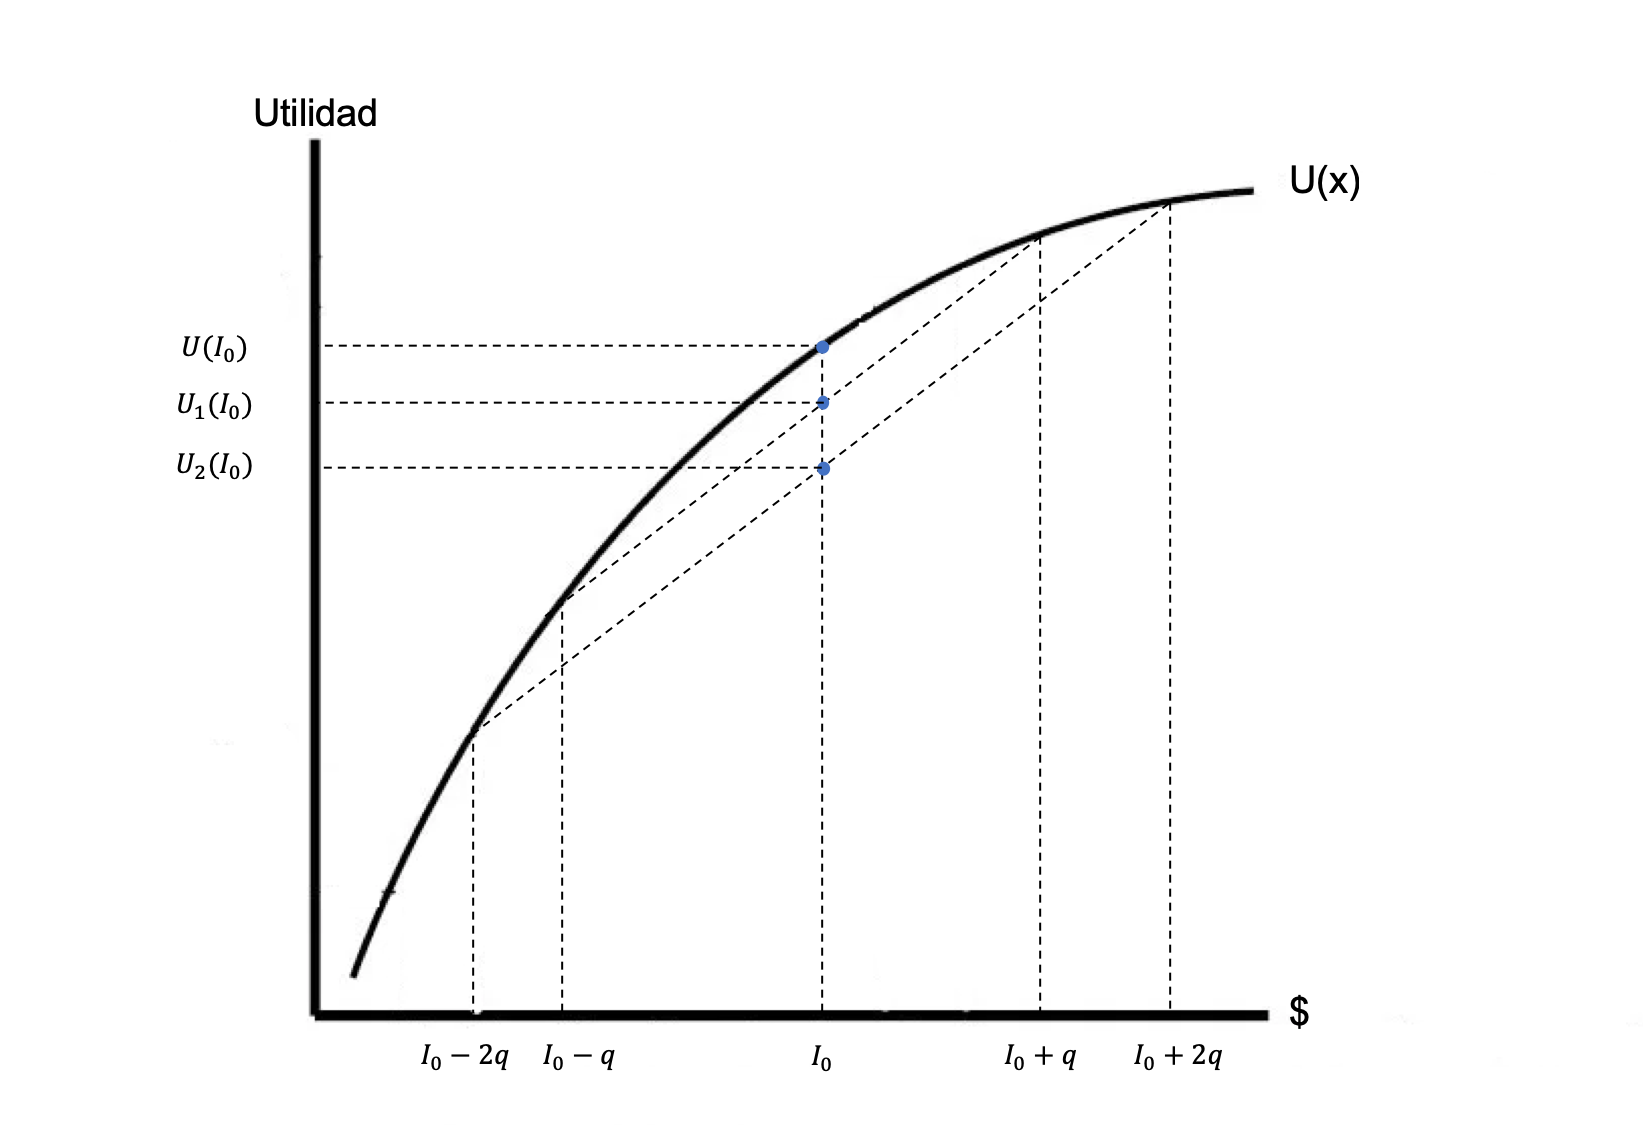
\includegraphics[scale = 0.43]{Imagenes/g1.png}
    \imagesource{Elaboración propia}
\end{figure}

Gráficamente podemos observar que:

$$
U(I_0) > U_{1}(I_0) > U_{2}(I_0)
$$

Con esto, podemos comprobar que un individuo averso al riesgo preferirá su riqueza inicial a jugar en una lotería justa y además preferirá una apuesta pequeña a una grande. También, se puede observar que cuando se tiene una riqueza menor, ganar el premio le genera mayor utilidad al individuo a comparación de la situación en donde la riqueza es mayor donde si se gana el premio la utilidad no aumenta de manera significativa. \\

Veamos un ejemplo numérico, supongamos que el indidividuo tiene una riqueza inicial $I_0 = \$100$ y se le propone apostar $\$80$ en un volado con una moneda honesta, por lo que la lotería quedaría definida de la siguiente manera:

\begin{table}[H]
\centering
\begin{tabular}{l|ll}
\cline{2-2}
    & x_1 = \$180 & con p_1 = \frac{1}{2} \\
L = &          &            \\
    & x_2 = \$20  & con p_2 = \frac{1}{2}  \\ \cline{2-2}
\end{tabular}
\end{table}

Observamos que, el valor esperado de la lotería $E[L] = \$100$ y tiene dos opciones:

\begin{itemize}
    \item No jugar y con probabilidad 1 tener $I_0 = \$100$ esto es $U(100)$
    \item Jugar la lotería y tener de utilidad esperada $UE[L] = p_1U(x_1) + p_2U(x_2)$ = $\frac{U(180)+U(20)}{2}$
\end{itemize} 

\newpage

Se tiene que, $U(100) > UE[L]$ esto debido a que al ser una función cóncava cualquier combinación lineal que se obtenga queda en el conjunto inferior dando una utilidad menor y por lo tanto prefiere no jugar. \\

Lo anterior se utilizará para comprobar que los individuos representativos que participan en estas loterías son aversos al riesgo y ver que tipo de loterías son (justas o injustas). Con ello se podrá entender de mejor manera si la decisión de participar o no en la lotería compensa el \textit{trade-off} entre el riesgo tomado y el valor esperado del premio potencial.

%VER SI ESTO LO DEJO O LO QUITO
%Por otro lado, supongamos a una persona que se enfrenta a una apuesta donde las probabilidades de ganar \$12 o perder \$10 son 50:50. El valor esperado es de \$1, la decisión de aceptar o no esta lotería involucra un \textit{trade-off}: aceptar la apuesta significa tomar riesgo, pero también implica un mayor valor esperado.

\newpage

\section{Aversión al riesgo y riqueza}

En la sección \textbf{1.1.3} se presenta la teoría de Arrow y Pratt donde se introduce una forma de medir cuantitativamente que tan averso al riesgo es un individuo. Con ello, surge la pregunta si la aversión al riesgo incrementa o disminuye dependiendo del nivel de riqueza con el que se cuenta. \\

Para poder dar una respuesta al cuestionamiento anterior, Arrow y Pratt presentan una familia de funciones para entender los cambios en la aversión al riesgo cuando la riqueza cambia. Respecto a  la medida de \textit{aversión al riesgo absoluto} existen 3 tipos de funciones:  CARA, DARA  y IARA las cuales presentan aversión al riesgo constante, decreciente y creciente respectivamente. \\

Algebráicamente lo anterior se obtiene de la derivada de la ecuación (1.6) para llegar a lo siguiente:

$$
r^{\prime}(W) = \left \{ \begin{matrix} <0  & \implies \mbox{DARA}
\\ = 0 & \implies \mbox{CARA} 
\\ >0 & \implies \mbox{IARA}

\end{matrix}\right.
$$ \\

Para entender de mejor forma esta familia de funciones, consideremos dos niveles de riqueza $W_1$ y $W_2$ con $W_1 > W_2$ y un posible pago monetario de $x$. Adicionalmente, supongamos $u(\cdot)$ una función de utilidad de tipo Bernoulli. \\

Un individuo con función de utilidad $u(\cdot)$ presenta aversión al riesgo absoluto decreciente (DARA) si:

\begin{equation}
    r(W_1 + x, u) < r(W_2 + x, u)
\end{equation}

Por otro lado, un individuo con función de utilidad $u(\cdot)$ presenta aversión al riesgo absoluto creciente (IARA) si:

\begin{equation}
    r(W_1 + x, u) > r(W_2 + x, u)
\end{equation}

Si tomamos ahora, una función de utilidad de la forma $u(W) = -e^{-\lambda W}$ con $\lambda > 0$ esta función de utilidad presenta aversión al riesgo absoluto constante (CARA) pues:

\begin{equation*}
    u^{\prime}(W)  & = \lambda e^{-\lambda W}, \: 
    u^{\prime \prime}(W) & = - \lambda^{2} e^{-\lambda W}
\end{equation*} 

\begin{equation*}
    \therefore r(W) = \lambda
\end{equation*}

Como se mencionó en la sección \textbf{1.1.3}, tratar de obtener estos coeficientes con los datos disponibles representa una dificultad dado que no se tiene una función de utilidad para cada individuo representativo de cada Estado y suponer una misma función de utilidad para todos no es lo ideal dado que no refleja la realidad. No se tomaría encuenta características ineherentes a cada Estado/Región que influyen en la percepción de la utilidad para cada individuo representativo. 

\newpage


\section{Elasticidades}
\noindent Una pregunta que se puede hacer en torno al ingreso y la cantidad demandada de un bien es cómo cambia el comportamiento de los individuos ante aumentos o disminuciones en el ingreso. ¿Consumirán más, menos o una cantidad igual de ese bien? \\

Para poder contestar la pregunta anterior defineremos a la elasticidad como \textit{una medida de sensibilidad que relaciona al precio o al ingreso con la cantidad demandada de un bien}. Utilizaremos este concepto debido a que, si bien es posible comparar las pendientes de diversas curvas de demanda, no siempre es lo óptimo puesto que estas pendientes dependen de las unidades en que medimos el precio y la cantidad y en ciertas ocasiones las unidades no están relacionadas. El concepto de elasticidad da la independecia de unidades. \\ 

Dentro de la teoría económica existen diferentes tipos de elasticidades, tales como: 

\begin{itemize}
    \item Elasticidad precio de la demanda
    \item Elasticidad precio de la oferta
    \item Elasticidad ingreso de la demanda
\end{itemize}

%per capita?
Para fines de esta tesis nos enfocaremos en la elasticidad ingreso para analizar los efectos y la sensibilidad existente entre la demanda de boletos del Sorteo Tec y el ingreso de los individuos representativos de cada Estado. Realizaremos un estudio similar a los que se describen en la sección \textbf{1.2 Revisión de literatura}. \\ 

Imaginemos dos situaciones, la primera donde la economía está en crecimiento y expansión, los individuos tienen ingresos más altos lo cual genera un aumento en la demanda de casi todos los bienes y servicios. La segunda, donde la economía se encuentra estancada o se empiezan a ver indicadores de que la economía empezará a decrecer, los individuos empiezan a tener menores ingresos lo cual genera una disminución en casi todos los bienes y servicios. \\

Para poder explicar que le pasará a la demanda de los bienes y servicios en ambas situaciones explicaremos a detalle la teoría asociada a las elasticidades. \\

La \textbf{elasticidad ingreso de la demanda}  es la medida de sensibilidad de la demanda de un bien ante un cambio en el ingreso, cuando los demás factores se mantienen constantes. Esta elasticidad se calcula de la siguiente forma:

$$
\varepsilon_I= \frac{ \Delta \% \: cantidad \: demandada}{\Delta \% \, ingreso}
$$

Dicha elasticidad ingreso puede ser positiva, negativa o cero:

\begin{itemize}
    \item $\varepsilon_I > 1$: bien \textit{superior} al ingreso
    \item $\varepsilon_I = 1$: bien con elasticidad ingreso unitaria
    \item $0 < \varepsilon_I < 1$: bien \textit{normal} al ingreso
    \item $\varepsilon_I = 0$: bien \textit{neutro} al ingreso
    \item $\varepsilon_I < 0$: bien \textit{inferior} al ingreso
\end{itemize}{}

Cuando un bien es superior al ingreso quiere decir que si el ingreso aumenta, la cantidad demandada aumenta en mayor proporción que el aumento en el ingreso. Cuando un bien es normal al ingreso quiere decir que si el ingreso aumenta, la cantidad demandada aumenta en menor proporción que el aumento en el ingreso y si un bien es inferior al ingreso, quiere decir que ante un aumento en el ingreso, la cantidad demandada de ese bien disminuye. \\

Así, buscaremos encontrar cuál es la elasticidad ingreso de los boletos del Sorteo Tec para determinar qué tipo de bien es. Esto se relacionará con la teoría de elección bajo incertidumbre y su relación con la teoría de utilidad esperada para poder determinar cómo es el comportamiento de los individuos representativos de cada Estado ante diferentes situaciones respecto al ingreso. \\



%====== Texto de la tesis de ejemplo
%\subsection{Cambios cerebrales y genéticos}

%\noindent Brizendine (2010) escribe que algunos científicos piensan que ciertas áreas del cerebro son como centros de actividad que mandan señales eléctricas a otras áreas del cerebro ocasionando un determinado comportamiento.\footnote{ Por ejemplo, en el hombre la corteza del cíngulo anterior pesa opciones, detecta conflicto y motiva decisiones. La unión temporoparietal busca soluciones rápidas y ante situaciones estresantes toma en cuenta la perspectiva de otros individuos. La corteza cingulada anterior rostral se encarga de procesar los errores sociales, como la aprobación o desaprobación de otros.}

%\begin{quote}
%    \small{Mientras que la distinción entre los cerebros de niños y niñas empieza biológicamente, estudios recientes muestran que es \textit{solo} el comienzo. La estructura cerebral no está escrita sobre piedra en el nacimiento ni al final de la infancia, como antes se creía, sino que continúa cambiando a lo largo de la vida. Más que ser inmutable, nuestros cerebros son mucho más plásticos y cambiables de lo que los científicos creían hace una década. El cerebro humano es también la máquina de aprendizaje más talentosa que conocemos. Así que nuestra cultura y el cómo nos enseñaron a comportarnos desempeñan un papel importante en el diseño y reestructura de nuestros cerebros (Brizendine 2010, 5-6).}
%\end{quote}

% Para citas muy largas es mejor el \begin{quote}

%\vspace{1em}
%\noindent \textbf{Hipótesis 3.} \hfill\begin{minipage}{\dimexpr\textwidth-3cm}
%\textit{La intensidad religiosa está relacionada negativamente con la innovación.}
%\end{minipage}
%\vspace{1em}

% Para plantear hipótesis

%\begin{table}[H]
%\centering
%\caption{Índices de modernidad y tradicionalismo}
%\label{PHEL}
%\begin{tabular}{|ccc|}
%\hline
% País & Índice de modernidad & Índice de tradicionalismo  \\ 
%\hline
%Alemania & 0.58 & 0.45 \\
%Austria & 0.55 & 0.49  \\
%Bélgica & 0.50 & 0.49  \\
%Canadá & 0.61 & 0.50 \\
%Dinamarca & 0.58 & 0.44 \\ 
%España & 0.47 & 0.62 \\
%Estados Unidos & 0.59 & 0.44  \\
%Finlandia & 0.62 & 0.38 \\
%Francia & 0.49 & 0.59 \\ 
%Holanda & 0.58 & 0.49 \\ 
%Irlanda & 0.54 & 0.59  \\
%Islandia & 0.63 & 0.54 \\
%Italia & 0.56 & 0.58  \\
%Japón & 0.42 & 0.48 \\
%Noruega & 0.53 & 0.44 \\
%Portugal & 0.50 & 0.71 \\ 
%Reino Unido & 0.56 & 0.54  \\
%Suecia & 0.62 & 0.51 \\
%Promedio & 0.58 & 0.51 \\
%\hline
%\end{tabular}

%\begin{tabular}{c}
%\footnotesize{Fuente: Bojilov y Phelps (2012).}
%\end{tabular}

%\end{table}

% Para diseñar tablas

%====== Acaba texto de tesis de ejemplo

\chapter{Modelo econométrico}

%\noindent Este capítulo tiene el propósito de probar empíricamente las hipótesis planteadas previamente y está dividido en dos secciones.


\section{Análisis exploratorio de datos}

\noindent Con apoyo del área de \textit{analytics} del Sorteo Tec se obtuvo la base de datos con la cual se trabajaron los modelos econométricos para obtener la elasticidad ingreso y las relaciones funcionales buscadas. Además de esto, se utilizó información publicada por el Instituto Nacional de Estadística y Geografía (INEGI) relacionada a los niveles del PIB por Estado así como los datos de los censos poblacionales. \\

Se nos proporcionó información de tres sorteos los cuales, a continuación se presenta una breve descripción\footnote{Consulta realizada en \textit{www.sorteostec.org} el 6 de abril de 2020}: 

\begin{itemize}
    
    \item \textbf{AventuraT}: el boleto tiene un precio de \$140. Los premios de este sorteo van desde un viaje alrededor del mundo con valor de \$1,000,000 hasta certificados para compras de productos del Sorteo Tec por valor de \$140.
    
    \item \textbf{Educativo}: el boleto tiene un precio de \$300. Los premios de este sorteo van desde un certificado por una carrera completa en el Tecnológico de Monterrey, premio en efectivo por \$12,000,000 hasta un premio de \$300.
    
    \item \textbf{Mi Sueño}: el boleto tiene un precio de \$600. Los premios de este sorteo son en efectivo/cheque los cuales van desde un premio de \$28,000,000 hasta un premio de \$600.
    
    
\end{itemize}

La información que hay en la base de datos proporcionada por el Sorteo Tec contiene datos de los tres sorteos mencionados anteriormente. Para cada sorteo se tiene el número de boletos vendidos por oficina en cada Estado y la fecha en la cual se celebró cada sorteo. \\

%11/10/2020

A continuación se presentan los Estados en los cuales se tiene registro de ventas de boletos del Sorteo Tec. Es importante mencionar que, no en todos los Estados del país existe un campus Tec de Monterrey pero, sí existen oficinas de representación en las cuales se pueden comprar boletos. La base de datos cuenta con información de 30 Estados y una oficina virtual, a los cuales se les asignó un ID y una variable indicadora si en dicho Estado hay un campus Tec de Monterrey. \\

\begin{table}[H]
\caption{Estados en donde se venden boletos del Sorteo Tec}
\label{edos}
\centering
\scalebox{0.8}{
\begin{tabular}{rrll}
  \hline
 ID & Estado & Campus \\ 
  \hline
  1 & Aguascalientes & Si \\ 
  2 & Baja California & No \\ 
  3 & Baja California Sur & No \\ 
  4 & Coahuila de Zaragoza & Si \\ 
  5 & Colima & Si \\ 
  6 & Chiapas & Si \\ 
  7 & Chihuahua & Si \\ 
  8 & Distrito Federal & Si \\ 
  9 & Durango & No \\ 
  10 & Guanajuato & Si \\ 
  11 & Guerrero & No \\ 
  12 & Hidalgo & Si \\ 
  13 & Jalisco & Si \\ 
  14 & Estado de Mexico & Si \\ 
  15 & Michoacan de Ocampo & Si \\ 
  16 & Morelos & Si \\ 
  17 & Nayarit & No \\ 
  18 & Nuevo Leon & Si \\ 
  19 & Oaxaca & No \\ 
  20 & Puebla & Si \\ 
  21 & Queretaro & Si \\ 
  22 & Quintana Roo & No \\ 
  23 & San Luis Potosi & Si \\ 
  24 & Sinaloa & Si \\ 
  25 & Sonora & Si \\ 
  26 & Tabasco & No \\ 
  27 & Tamaulipas & Si \\ 
  28 & Veracruz de Ignacio de la Llave & Si \\ 
  29 & Yucatan & No \\ 
  30 & Zacatecas & Si \\ 
  31 & Oficina Virtual & No \\ 
   \hline
\end{tabular}
}
\end{table}


Se transformó esta información para poder llegar al número de boletos vendidos por Estado. A continuación, a manera de ejemplo, se presentan las primeras seis observaciones de la tabla que resulta del manejo de datos para el sorteo AventuraT:

\begin{table}[H]
\caption{Datos para el sorteo AventuraT}
\label{aven}
\scalebox{0.8}{
\begin{tabular}{ccccccc}
\hline
\multicolumn{1}{l}{Estado}              & \multicolumn{1}{1}{ID} & \multicolumn{1}{l}{Fecha} & \multicolumn{1}{l}{\# Boletos} & \multicolumn{1}{l}{PIB \textit{per capita} } & \multicolumn{1}{l}{PIB*} & \multicolumn{1}{1}{Campus} \\ \hline
Aguascalientes                          & 1  & 4/dic/2015                & 553                            & 150,985.72                 & 198,175.39               & Sí     \\
Baja California                         & 2  & 4/dic/2015                & 1498                           & 152,585.45                 & 505,937.66               & No     \\
Baja California Sur                     & 3  & 4/dic/2015                & 953                            & 182,712.47                 & 130,096.58               & No     \\
Coahuila de Zaragoza                    & 4  & 4/dic/2015                & 4650                           & 194,201.89                 & 573,850.07               & Sí     \\
Colima                                  & 5  & 4/dic/2015                & 1725                           & 134,073                    & 95,357.74                & Sí     \\
Chiapas                                 & 6  & 4/dic/2015                & 389                            & 55,666                     & 290,463.61               & Sí     \\ \hline
\multicolumn{1}{l}{*Cifras en millones de pesos} &    &                           &                                &                            &                          &        \\ 
\end{tabular}
}
\centering
\source{Fuente: Elaboración propia con datos del Sorteo Tec}

\end{table} \\

Con la información obtenida para cada sorteo se realizaron diferentes visualizaciones para obtener mayor información acerca de los datos. En primer lugar se presenta un diagrama de cajas y brazos, diferenciando en grupos si existe un campus Tec de Monterrey en el Estado, en donde se observa que para los 3 sorteos los Estados que más boletos vendieron entre 2015 y 2019 son Nuevo León, Tamaulipas, Jalisco y la Oficina Virtual. En estos primeros 3 estados existe un campus Tec de Monterrey, lo cual puede darnos una idea si el hecho de que exista un campus en el Estado tenga un efecto sobre el número de boletos vendidos.

\begin{figure}[H]
    \caption{Boletos vendidos por Estado}
    \label{fig:boxplot}
    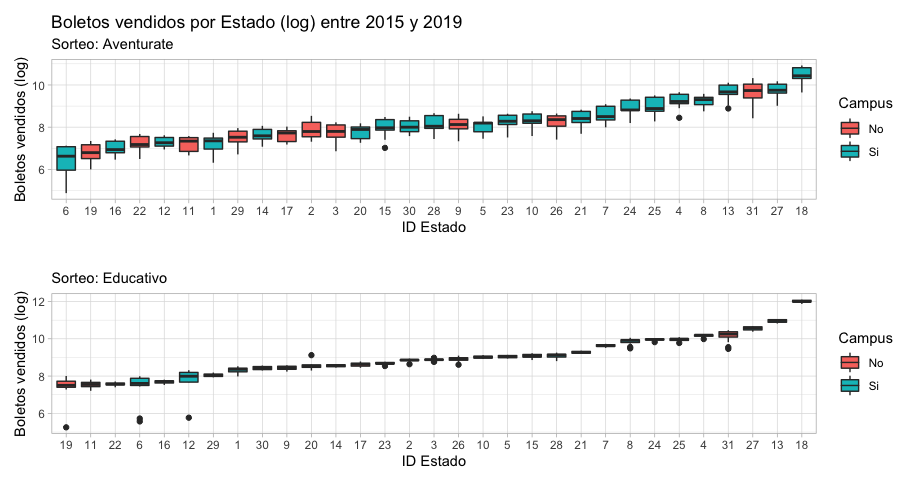
\includegraphics[scale = 0.43]{Imagenes/boxplot1.png}
    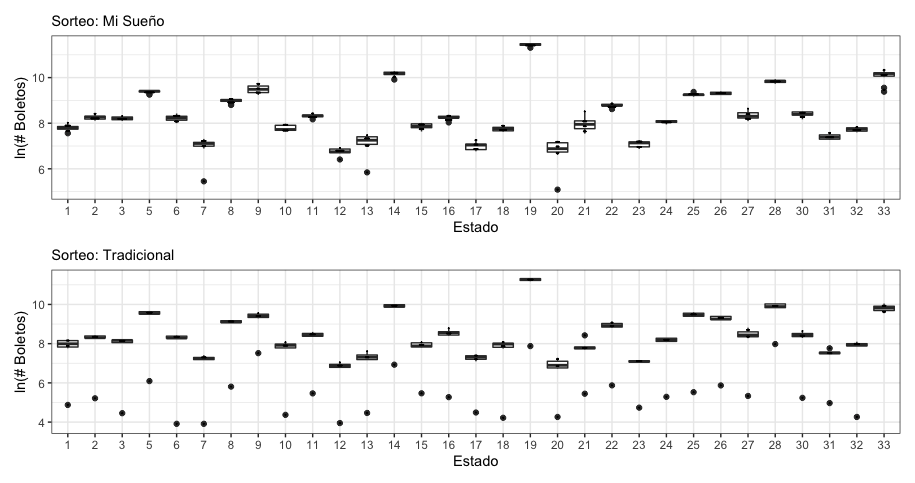
\includegraphics[scale = 0.43]{Imagenes/boxplot2.png}
    \centering
    \imagesource{Elaboración propia}
\end{figure}


En relación a lo anterior, se presenta la matriz de correlaciones entre las variables: 

\begin{itemize}
    \item \textit{campus}: variable indicadora si existe un campus en el Estado o no.
    \item \textit{pib\_pc}: PIB \textit{per capita} por Estado en escala logarítimica. \\
    \item \textit{n\_boletos}: número de boletos vendidos por Estado en escala logarítmica.
\end{itemize} \\

\begin{figure}[H]
    \caption{Matriz de Correlación por Sorteo}
    \label{fig:corplot}
    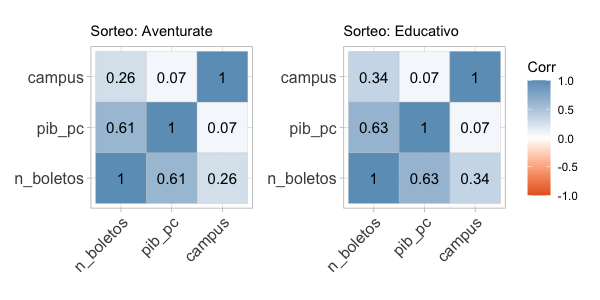
\includegraphics[scale = 0.4]{Imagenes/cp1.png} \\
    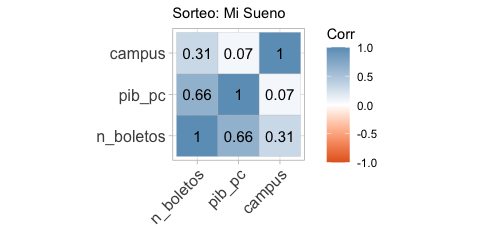
\includegraphics[scale = 0.5]{Imagenes/cp2.png} \\
    \centering
    \imagesource{Elaboración propia}
\end{figure} 

Se observa que para los 3 sorteos hay una correlación positiva alta entre las variables \textit{n\_boletos} y \textit{pib\_pc}, mientras que la correlación entre las variables \textit{campus} y \textit{n\_boletos} si bien es positiva no tiene un nivel alto a excepción en los sorteos Educativo y Mi Sueño. \\

Por otro lado, se analizó la variable de boletos vendidos por Estado. Primero observamos que el sorteo Educativo es el que más boletos ha vendido entre 2015 y 2019, esto se podría explicar debido a que cierto grupo de alumnos de la institución tienen que vender cierta cantidad de boletos ligado a alguna ayuda financiera que la Institución les esté otorgando.
    
\begin{figure}[H]
    \caption{Boletos vendidos por sorteo}
    \label{fig:bolvendidos}
    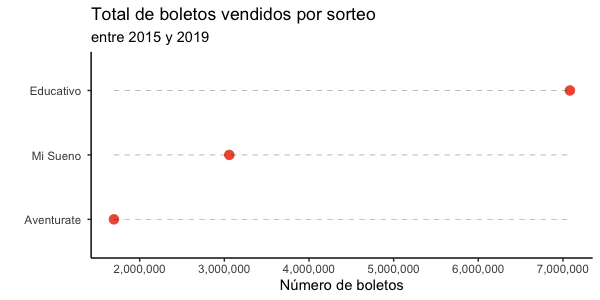
\includegraphics[scale = 0.5]{Imagenes/n_boletos.png} \\
    \centering
    \imagesource{Elaboración propia}
\end{figure} 

Ahora bien, observamos esta misma información pero agrupada de diferente manera. Agrupamos el número de boletos vendidos por Estado y observamos que entre 2015 y 2019 el Estado que vendió más boletos fue Nuevo León. Esto se podría explicar debido a que la Institución nace en este Estado y la presencia del número de docentes, alumnos y personal es significativamente mayor en comparación a otros Estados. Si bien, como se observó en la figura 3.2 la correlación entre que haya un campus en el Estado no tiene una correlación positiva elevada, se observa en las siguientes gráficas que para todos los sorteos los Estados que más boletos venden son los que tienen un campus Tec de Monterrey.

\begin{figure}[H]
    \caption{Boletos vendidos por Estado}
    \label{fig:bolvendidos}
    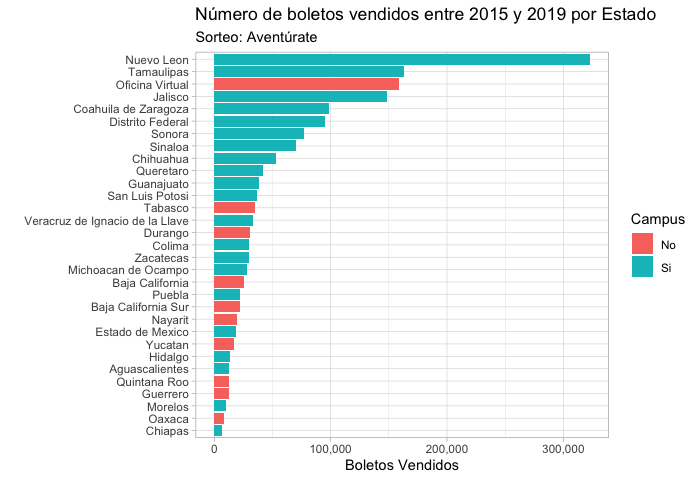
\includegraphics[scale = 0.5]{Imagenes/boletos_av.png} \\
    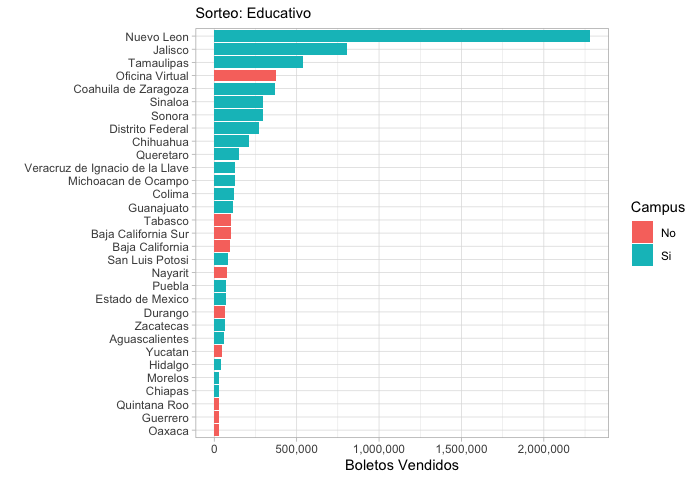
\includegraphics[scale = 0.5]{Imagenes/boletos_ed.png} \\
    \centering
%    \imagesource{Elaboración propia}
\end{figure} \\

\begin{figure}[H]
%    \caption{Boletos vendidos por Estado}
    \label{fig:bolvendidos2}
    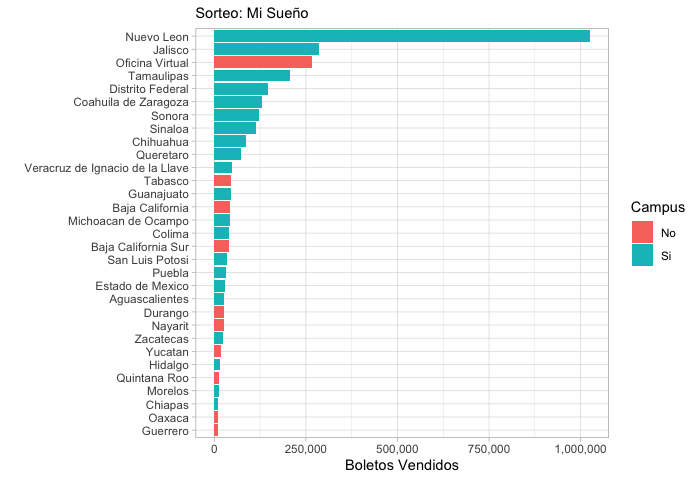
\includegraphics[scale = 0.5]{Imagenes/boletos_sue.png} \\
    \centering
     \imagesource{Elaboración propia}
\end{figure} 

De igual forma, se observaron los 15 Estados que vendieron más boletos entre 2015 y 2019 para analizar como se comportaron las ventas en cada fecha de sorteo. Para el sorteo Aventúrate se observa una tendencia creciente en el número de boletos vendidos  y apartir de 2018 se ve una clara disminución para los 15 Estados. Para los otros 2 sorteos no se observa una tendencia clara. Es importante mencionar que, en la selección de estas 15 entidades se observan Estados que no cuentan con un campus Tec de Monterrey en él.

\begin{figure}[H]
    \caption{Estados que más boletos vendieron}
    \label{fig:bolvendidos_top}
    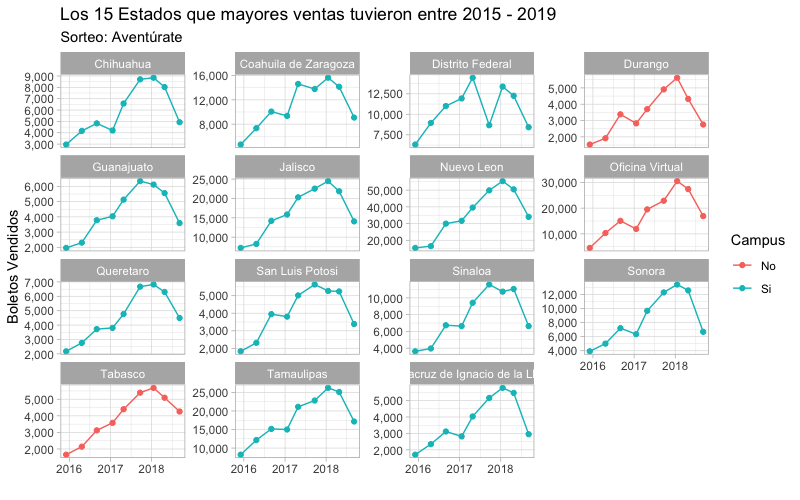
\includegraphics[scale = 0.5]{Imagenes/aven_15edos.png} \\
    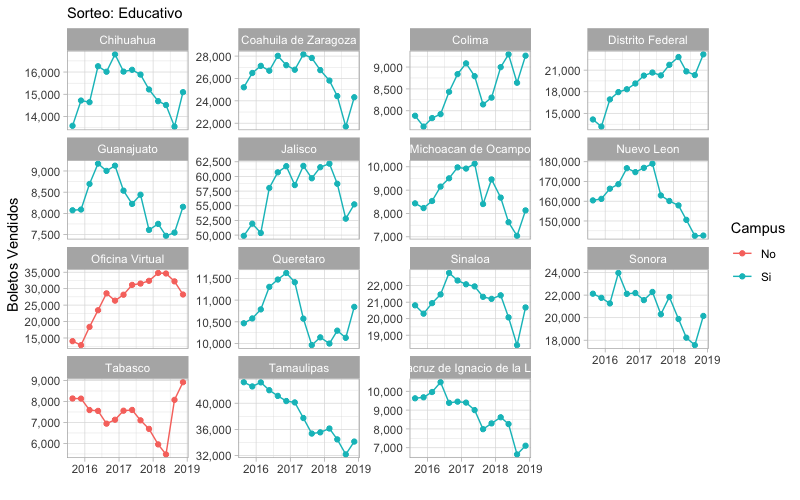
\includegraphics[scale = 0.5]{Imagenes/educ_15edos.png} \\
    \centering
%    \imagesource{Elaboración propia}
\end{figure} \\

\begin{figure}[H]
%    \caption{Boletos vendidos por Estado}
    \label{fig:bolvendidos_top2}
    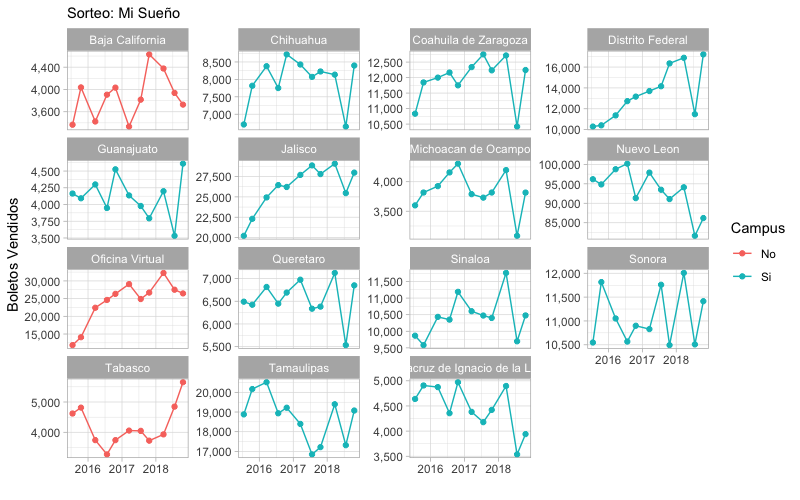
\includegraphics[scale = 0.5]{Imagenes/sue_15edos.png} \\
   % 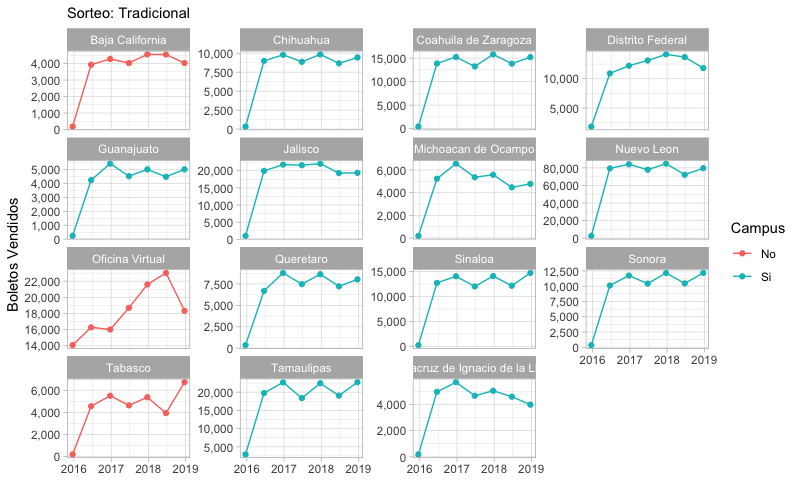
\includegraphics[scale = 0.5]{Imagenes/trad_15edos.png} \\
    \centering
    \imagesource{Elaboración propia}
\end{figure} 

Por otro lado, se buscó encontrar la relación existente entre el número de boletos vendidos y el PIB \textit{per capita} (aplicando logaritmos a las dos variables para cada sorteo). Esto con la intención de analizar más a fondo lo observado en la figura 3.2.

\begin{figure}[H]
    \caption{Boletos vs PIB \textit{per capita} (log - log)}
    \label{fig:scat}
    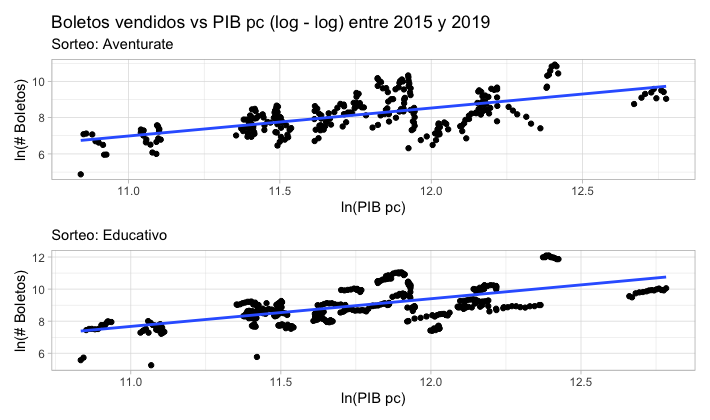
\includegraphics[scale = 0.35]{Imagenes/sc1.png}
    \centering
    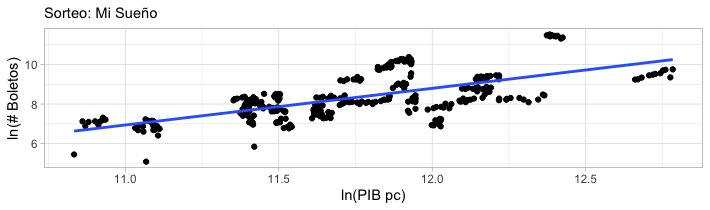
\includegraphics[scale = 0.35]{Imagenes/sc2.png} \\
    \centering
    \imagesource{Elaboración propia}
\end{figure}

De las gráficas anteriores, se observa una clara relación positiva entre el logaritmo natural del número de boletos vendidos y el logaritmo natural del PIB \textit{per capita}. Esto resulta relevante pues, como se mencionó en el capítulo anterior, la elasticidad ingreso nos mide la sensibilidad en la cantidad demandada de un bien cuando cambia el ingreso. Observar esta relación positiva nos empieza a dar señales de cómo será esta elasticidad. \\

%Por otro lado, observamos que para los cuatro sorteos el Estado en donde se registraron el mayor número de boletos vendidos fue Nuevo León. Un aspecto relevante es que entre los años 2015 y 2019 Nuevo León fue el tercer Estado con un PIB promedio más alto como se ve en la siguiente gráfica.

%\begin{figure}[H]
%    \centering
%    \caption{PIB por Estado}
%    \label{fig:box-pib}
%    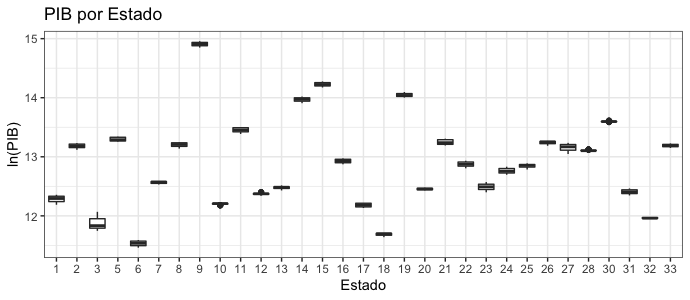
\includegraphics[scale = 0.5]{Imagenes/boxplot_pib.png}
%    \imagesource{Elaboración propia}
%\end{figure}





\newpage

\section{Modelo}

\noindent Para la comprobación de la hipótesis propuesta para esta tesis, se corrieron diferentes modelos de regresión tanto log-log como múltiple. \\

Los modelos econométricos que se utilizarán en este trabajo son los siguientes:

\begin{equation}
    ln(y) = \beta_0 + \beta_1 ln(x) + \epsilon
\end{equation}

\begin{equation}
    y = \alpha_0 + \alpha_1 x + \alpha_2 x^2 + \epsilon
\end{equation}
 
Donde $y$ es el número de boletos vendidos, $x$ es el PIB \textit{per capita} y $\epsilon \sim N(0,\sigma^2)$ para ambos modelos. Estos modelos nos servirán para encontrar con la ecuación (3.1) la elasticidad ingreso y con la ecuación (3.2) la concavidad de la función. \\

El modelo (3.1) se origina de la siguiente manera. Consideremos el siguiente modelo que se conoce como \textit{regresión exponencial}:

\begin{equation}
    Y_i = \theta_0 X_{i}^{\beta_1} e^{u_i}
\end{equation}

El cual puede ser expresado de la siguiente forma:

\begin{equation}
    ln (Y_i) = \beta_0 + \beta_1 ln (X_i) + u_i
\end{equation}

Donde $\beta_0 = ln (\theta_0)$. A la ecuación (3.4) se le conoce como \textbf{modelo log-log}, este modelo resulta ser lineal en los parámetros $\beta_0$ y $\beta_1$, lineal en los logaritmos de las variables Y y X. De aquí se sigue que, si los supuestos de una regresión lineal clásica se cumplen, los parámetros pueden ser estimados mediante mínimos cuadrados ordinarios sustituyendo $Y_i^* = ln (Y_i)$ y $X_i^* = ln(X_i)$ llegando a la siguiente ecuación:

\begin{equation}
    Y_i^* = \beta_0 + \beta_1X_i^* + u_i
\end{equation}

Se propone el modelo log-log debido a que el coeficiente $\beta_1$ mide la elasticidad de Y respecto a X. Es importante mencionar que, el modelo asume que la elasticidad es constante a través de toda la curva, en otras palabras esto significa que el cambio en $ln(Y)$ debido al cambio en $ln(X)$ permanece constante sin importar a que nivel de $ln(X)$ se esté midiendo la elasticidad. \\

Traduciéndolo a nuestro contexto, si tomamos el modelo (3.1) con nuestras variables tenemos que:

\begin{equation}
    \beta_1 = \frac{\Delta \: \% \:boletos \: vendidos}{\Delta \: \% \: PIB \: pc} \equiv \varepsilon_{I,x}
\end{equation} \\


Así, obtenemos la elasticidad ingreso de los boletos del Sorteo Tec la cual es parte central de nuestra investigación. \\

Ahora, el modelo (3.2) nos explicará si existe una forma funcional cóncava o convexa, esto se obtiene del coeficiente $\alpha_2 = \frac{\partial^2 y}{\partial x^2}$ del cual nos interesa el signo. Traduciéndolo a nuestro contexto con nuestras variables, tenemos que:

\begin{equation}
    \alpha_2 = \frac{\partial^2 \:boletos \: vendidos}{\partial PIB \: pc^2}
\end{equation}

Si $\alpha_2 < 0$ tenemos una función cóncava y si $\alpha_2 > 0$ tenemos una función convexa. Bajo nuestra hipótesis, esperaríamos que la función fuera cóncava lo cual nos daría una idea de que el individuo es averso al riesgo como se explicó en el capítulo \textbf{2.1}. \\

Estos modelos se utilizarán para los 3 sorteos y así analizar cada uno por separado. A continuación, en el \textbf{cuadro 3.3} se presenta el ajuste que se realizó para el modelo (3.1) y en el \textbf{cuadro 3.4} se presenta el ajuste que se realizó para el modelo (3.2). El ajuste se realizó con el método de mínimos cuadrados ordinarios y se utilizó el software estadístico R. La validación de los modelos se encuentra en los apéndices A y B. \\

%Regresiones para los 4 sorteos: modelo ln(y) ~ ln(x)

\begin{table}[H] 
\centering 
  \caption{Ajuste Modelo (3.1)} 
  \label{lm_loglog} 
\scalebox{0.65}{
\begin{tabular}{@{\extracolsep{5pt}}lccc} 
\\[-1.8ex]\hline 
\hline \\[-1.8ex] 
 & \multicolumn{3}{c}{\textit{Dependent variable:}} \\ 
\cline{2-4} 
\\[-1.8ex] & \multicolumn{3}{c}{log(Venta Estado)} \\ 
\\[-1.8ex] & (AventuraT) & (Educativo) & (Mi Sueño)\\ 
\hline \\[-1.8ex] 
 log(PIB \textit{per capita}) & 1.542$^{***}$ & 1.726$^{***}$ & 1.854$^{***}$ \\ 
  & (0.120) & (0.103) & (0.113) \\ 
  & & & \\ 
 Constant & $-$9.979$^{***}$ & $-$11.317$^{***}$ & $-$13.448$^{***}$ \\ 
  & (1.417) & (1.211) & (1.335) \\ 
  & & & \\ 
\hline \\[-1.8ex] 
R$^{2}$ & 0.372 & 0.395 & 0.441 \\ 
Adjusted R$^{2}$ & 0.370 & 0.393 & 0.440 \\ 
Residual Std. Error & 0.809 (df = 277) & 0.861 (df = 431) & 0.835 (df = 338) \\ 
F Statistic & 163.937$^{***}$ (df = 1; 277) & 281.194$^{***}$ (df = 1; 431) & 266.968$^{***}$ (df = 1; 338) \\ 
\hline 
\hline \\[-1.8ex] 
\textit{Note:}  & \multicolumn{3}{r}{$^{*}$p$<$0.1; $^{**}$p$<$0.05; $^{***}$p$<$0.01} \\ 
\end{tabular} 
}
\end{table} 

%Regresiones para los 4 sorteos: modelo y ~ x + x^2

\begin{table}[H] 
\centering 
  \caption{Ajuste Modelo (3.2)} 
  \label{cuadratic_model} 
\scalebox{0.65}{
\begin{tabular}{@{\extracolsep{5pt}}lccc} 
\\[-1.8ex]\hline 
\hline \\[-1.8ex] 
 & \multicolumn{3}{c}{\textit{Dependent variable:}} \\ 
\cline{2-4} 
\\[-1.8ex] & \multicolumn{3}{c}{Venta Estado} \\ 
\\[-1.8ex] & (AventuraT) & (Educativo) & (Mi Sueño)\\ 
\hline \\[-1.8ex] 
 PIB \textit{per capita} & 0.120$^{***}$ & 0.418$^{***}$ & 0.221$^{***}$ \\ 
  & (0.028) & (0.084) & (0.054) \\ 
  & & & \\ 
  
 (PIB \textit{per capita})^2 & $-$1.613e-07$^{**}$ & $-$5.713e-07$^{**}$ & $-$2.588e-07$^{*}$  \\ 
  & (7.606e-08) & (2.291e-07) & (1.471e-07) \\ 
  & & & \\ 
 Constant & $-$6,909.530$^{***}$ & $-$28,626.400$^{***}$ & $-$15,784.160$^{***}$ \\ 
  & (2,285.693) & (6,858.514) & (4,410.503) \\ 
  & & & \\ 
\hline \\[-1.8ex] 
R$^{2}$ & 0.222 & 0.194 & 0.208 \\ 
Adjusted R$^{2}$ & 0.216 & 0.191 & 0.204 \\ 
Residual Std. Error & 7,136.310 (df = 276) & 26,589.100 (df = 430) & 15,011.720 (df = 337) \\ 
F Statistic & 39.377$^{***}$ (df = 2; 276) & 51.861$^{***}$ (df = 2; 430) & 44.358$^{***}$ (df = 2; 337) \\ 
\hline 
\hline \\[-1.8ex] 
\textit{Note:}  & \multicolumn{3}{r}{$^{*}$p$<$0.1; $^{**}$p$<$0.05; $^{***}$p$<$0.01} \\ 
\end{tabular}  
}
\end{table} \\

Como comentario adicional, se ajustaron dos modelos más, al modelo 3.1 y al modelo 3.2 se les agregó una variable indicadora que corresponde a la existencia de un campus Tec en el Estado, esto con la intención de ver el efecto fijo que podría presentar tanto en la estimación de la elasticidad como en la concavidad de la función. Los resultados de dicho ajuste no presentaron diferencias significativas a los presentados en las tablas anteriores (se preservaron las magnitudes y los signos).


% Para escribir ecuaciones

%\begin{table}[H]
%\centering
%\caption{Resultados del modelo econométrico}
%\label{REG}
%\begin{tabular}{|ccccc|}
%  \hline
% & Estimador & Desv. est. & Valor $t$ & Pr($>|t|$) \\ 
%  \hline
%  $\alpha$ & x & x & x & x \\ 
%  CI & x & x & x & x \\ 
%  IS & x & x & x & x \\ 
%  IR & x & x & x & x \\ 
%  PT & x & x & x & x \\ 
%   \hline
%\multicolumn{5}{|c|}{Error est. de res. = x con x gr. de libertad}
%    \\
%    \multicolumn{5}{|c|}{$R^2$ = x y $\bar{R}^2$ = x}
% \\
% \multicolumn{5}{|c|}{Estadístico $F$ = x, con un valor $p$ = x }
%      \\
%\hline
%\end{tabular} \\

%\end{table}


\chapter{Resultados}

%\noindent En este último capítulo se analiza los resultados del caso del Sorteo Tec en dos partes: la dimensión nacional y la internacional. 

\newpage

\section{El Sorteo Tec}

%Analisis de valor esperado de los diferentes sorteos

\noindent A continuación, pasaremos al análisis de aversión al riesgo de las diferentes loterías. Se cuenta con la información relacionada al número de premios, el valor de los premios y el número de boletos emitidos en cada sorteo, con esta información se obtuvieron las probabilidades asociadas a cada premio y así definir la lotería $L$ como se mencionó en el capítulo \textbf{2.1}. \\

Para el sorteo \textbf{AventuraT} se tiene una emisión de 60,000 boletos y hay un total de 6,421 premios. Con esta información sabemos que la probabilidad de ganar alguno de los premios es de 0.10702.

\begin{table}[H]
\centering
\caption{Información sorteo AventuraT}
\label{tab:avent}
\begin{tabular}{@{}lll@{}}
\toprule
\multicolumn{1}{c}{Premios} & \multicolumn{1}{c}{\$} & \multicolumn{1}{c}{Probabilidad} \\ \midrule
1                           & 1,000,000                & 0.00001666666667                 \\
1                           & 100,000                 & 0.00001666666667                 \\
1                           & 50,000                  & 0.00001666666667                 \\
3                           & 20,000                  & 0.00005                          \\
10                          & 5,000                   & 0.0001666666667                  \\
25                          & 2,500                   & 0.0004166666667                  \\
80                          & 1,000                   & 0.001333333333                   \\
300                         & 500                    & 0.005                            \\
6,000                        & 140                    & 0.1                              \\ \bottomrule
\end{tabular}
\end{table}

Además, se obtuvo el valor esperado de esta lotería. El resultado fue $E[L] =$ 39.88, menor al valor del boleto que es de $\$ 140$. \\ \\\\

Para el sorteo \textbf{Educativo} se tiene una emisión de 470,000 y un total de 26, 835 premios. Con esta información sabemos que la probabilidad de ganar alguno de los premios es de 0.05710

\begin{table}[H]
\centering
\caption{Información sorteo Educativo}
\label{tab:educ}
\begin{tabular}{@{}lll@{}}
\toprule
\multicolumn{1}{c}{Premios} & \multicolumn{1}{c}{\$} & \multicolumn{1}{c}{Probabilidad} \\ \midrule
1                           & 12,000,000               & 0.000002127659574                \\
2                           & 1,045,000                & 0.000004255319149                \\
7                           & 1,000,000                & 0.00001489361702                 \\
10                          & 100,000                 & 0.00002127659574                 \\
15                          & 50,000                  & 0.00003191489362                 \\
100                         & 5,000                   & 0.0002127659574                  \\
400                         & 2,500                   & 0.0008510638298                  \\
2,800                        & 1,000                   & 0.005957446809                   \\
23,500                       & 300                    & 0.05                             \\ \bottomrule
\end{tabular}
\end{table}

\newpage
Para el sorteo \textbf{Mi Sueño} se tiene una emisión de 280,000 boletos y hay un total de 19,950 premios. Con esta información sabemos que la probabilidad de ganar alguno de los premios es de 0.07125. 

\begin{table}[H]
\centering
\caption{Información sorteo Mi Sueño}
\label{tab:misuen}
\begin{tabular}{@{}lll@{}}
\toprule
\multicolumn{1}{c}{Premios} & \multicolumn{1}{c}{\$} & \multicolumn{1}{c}{Probabilidad} \\ \midrule
1                           & 28,000,000               & 0.000003571428571        \\
1                           & 5,333,280                & 0.000003571428571        \\
1                           & 1,800,000                & 0.000003571428571        \\
7                           & 100,000                 & 0.000025                 \\
10                          & 50,000                  & 0.00003571428571         \\
50                          & 10,000                  & 0.0001785714286          \\
280                         & 5,000                   & 0.001                    \\
2,800                        & 1,650                   & 0.01                     \\
5,600                        & 1,100                   & 0.02                     \\
11,200                       & 600                    & 0.04                     \\ \bottomrule
\end{tabular}
\end{table} \\

Además, con esta información podemos obtener el valor esperado de esta lotería. Así obtenemos que $E[L] = $ 199.05, menor al valor del boleto que es de $\$ 600$. 

\newpage
Para el sorteo \textbf{Tradicional} se tiene una emisión de 250,000 boletos y un total de 12,323 premios. Con esta información sabemos que la probabilidad de ganar alguno de los premios es de 0.04929.

\begin{table}[H]
\centering
\caption{Información sorteo Tradicional}
\label{tab:trad}
\begin{tabular}{@{}lll@{}}
\toprule
\multicolumn{1}{c}{Premios} & \multicolumn{1}{c}{\$} & \multicolumn{1}{c}{Probabilidad} \\ \midrule
1                           & 60,750,000               & 0.000004                         \\
1                           & 8,500,000                & 0.000004                         \\
1                           & 3,226,000                & 0.000004                         \\
1                           & 1,100,000                & 0.000004                         \\
1                           & 949,900                 & 0.000004                         \\
1                           & 841,000                 & 0.000004                         \\
1                           & 719,900                 & 0.000004                         \\
1                           & 495,000                 & 0.000004                         \\
80                          & 100,000                 & 0.00032                          \\
100                         & 20,000                  & 0.0004                           \\
400                         & 5,000                   & 0.0016                           \\
1,735                        & 2,500                   & 0.00694                          \\
10,000                       & 1,100                   & 0.04                             \\ \bottomrule
\end{tabular}
\end{table}

Además, como esta información podemos obtener el valor esperado de esta lotería. Así obtenemos que $E[L] = $ 415.68, menor al valor del boleto que es de $\$ 1100$. \\

%Esto no estoy muy seguro de dejarlo
\newpage

Ahora bien, el valor esperado de cada lotería y las probabilidades que hay de ganar un premio nos hacen remarcar lo siguiente: las apuestas con probabilidad de ganar ($p$) pequeñas resultan menos atractivas de lo que deberían para un individuo que maximiza su utilidad. De aquí que la forma en que se utilizan los pesos para calcular tanto el valor esperado como la utilidad esperada generan una fuente de aversión al riesgo (O’Donoghue y Somerville, 2018). \\

Por otro lado, la aversión al riesgo deriva de la utilidad marginal decreciente que existe por la riqueza monetaria. Supongamos a dos individuos con diferentes riquezas tales que la riqueza de uno es mayor que del otro. Sea $W_a$ y $W_b$ las riquezas para los individuos A y B respectivamente y que $W_a < W_b$, además bajo el supuesto que estos dos individuos son aversos al riesgo la utilidad que le daría ganar un premio al individuo A es mayor a la utilidad que le daría ganar un premio al individuo B. \\

\newpage

Esto se debe a la concavidad de la función de utilidad que representa a los individuos aversos al riesgo, la pendiente en el punto $M$ es mayor a la pendiente en el punto $N$ y esto nos explica la forma en que la utilidad aumenta en cada caso. Gráficamente se ve de la siguiente manera:

\begin{figure}[H]
    \centering
    \caption{Comparación dos individuos}
    \label{fig:my_label}
    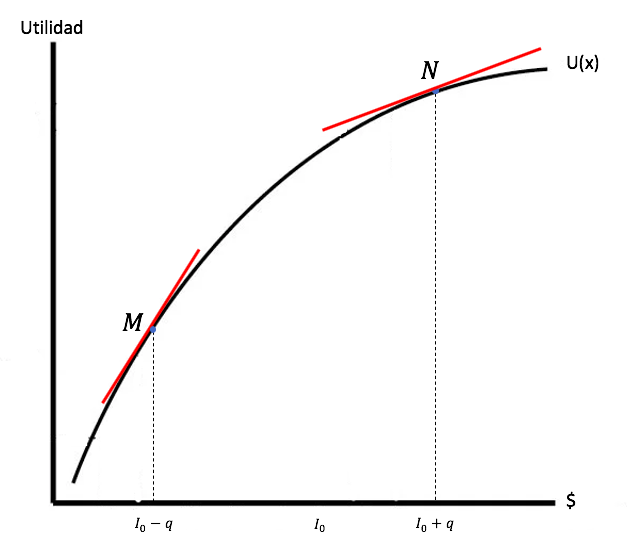
\includegraphics[width=.85\linewidth]{Imagenes/UE_MN.png} \\
    \imagesource{Elaboración propia}
\end{figure}




\newpage
%%Analisis de resultados del modelo econometrico

Pasemos ahora a analizar los resultados obtenidos de nuestros modelos. Como mencionamos en el capítulo anterior, los coeficientes relevantes resultan ser $\beta_1$ para el modelo (3.1) y $\beta_2$ para el modelo (3.2). Retomemos los resultados obtenidos de estos modelos:

\begin{table}[H]
\centering
\caption{Resumen coeficientes}
\label{tab:my-table}
\begin{tabular}{lcccc}
\hline
      & \multicolumn{1}{l}{AventuraT} & \multicolumn{1}{l}{Educativo} & \multicolumn{1}{l}{Mi sueño} & \multicolumn{1}{l}{Tradicional} \\ \hline
\multicolumn{5}{c}{Modelo (3.1)}                                                                                                       \\
\beta_1 & 1.542                         & 1.726                         & 1.854                        & 1.751                           \\ \hline
\multicolumn{5}{c}{Modelo (3.2)}                                                                                                       \\
\beta_2 & $-$1.613e-07 & $-$5.713e-07  & $-$2.588e-07   & $-$2.253e-07 \\              
\end{tabular}
\end{table}

Observamos que, para todos los sorteos el coeficiente $\beta_1 > 1$ lo que nos indica que las elasticidad ingreso de los boletos del Sorteo Tec es mayor a uno. Por otro lado, todos los coeficientes fueron estadísticamente diferentes de 0 a excepción de $\beta_2$ para el sorteo Tradicional. \\

\begin{equation*}
     \beta_1 > 1
\end{equation*}
\begin{equation*}
    \Rightarrow \varepsilon_{I,x} > 1
\end{equation*}
\begin{equation*}
    \Rightarrow \frac{\Delta\% Boletos}{\Delta \% PIB pc} >1
\end{equation*} 

\newpage

Esto nos indica que el bien es un \textbf{bien superior al ingreso}, lo cual se traduce que ante un cambio en el PIB \textit{per capita} el cambio en el número de boletos será mayor en valor absoluto. Este resultado va en línea con nuestra hipótesis, sustentando nuestra idea inicial que ante disminuciones en el ingreso la cantidad demanda de boletos disminuye. Esto aplica para los cuatro sorteos sobre los cuales se realizó el análisis.  \\

\begin{table}[H]
\centering
\begin{tabular}{l|ll}
\cline{1-1}
\downarrow I \Rightarrow \ \downarrow X  &   &   \\
          & = & \mid \Delta X| > |\Delta I| \\
\uparrow I \Rightarrow \ \uparrow X &   &   \\ \cline{1-1}
\end{tabular}
\end{table} 

\begin{figure}[H]
\centering
\caption{Relación \beta_1}
\label{fig:test}
\begin{subfigure}
  \centering
  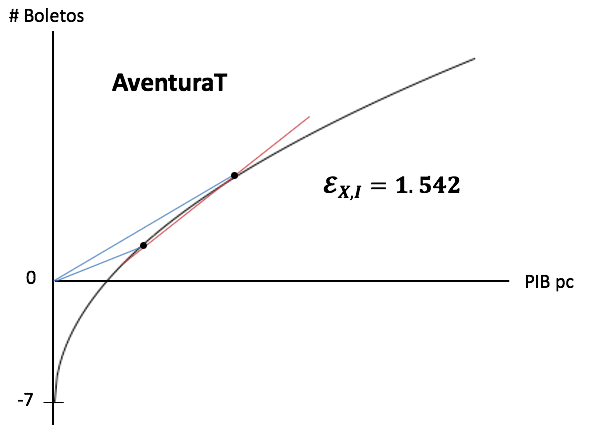
\includegraphics[width=.45\linewidth]{Imagenes/aven.png}
\end{subfigure}%
\begin{subfigure}
  \centering
  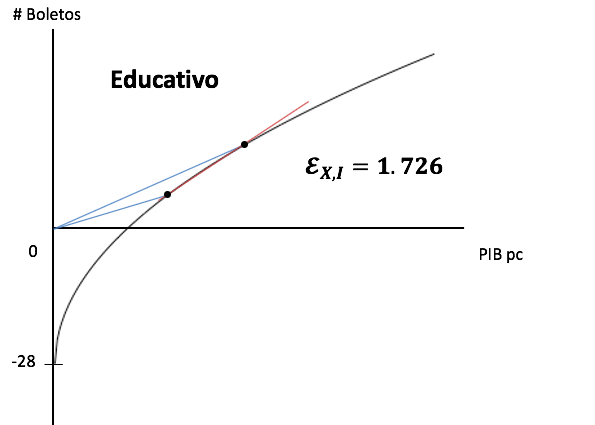
\includegraphics[width=.45\linewidth]{Imagenes/educ.png}
\end{subfigure}
\end{figure}

\begin{figure}[H]
\centering
\begin{subfigure}
  \centering
  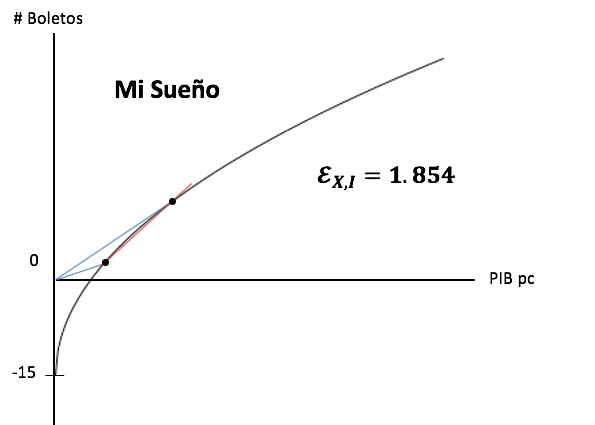
\includegraphics[width=.45\linewidth]{Imagenes/suen.png}
\end{subfigure}%
\begin{subfigure}
  \centering
  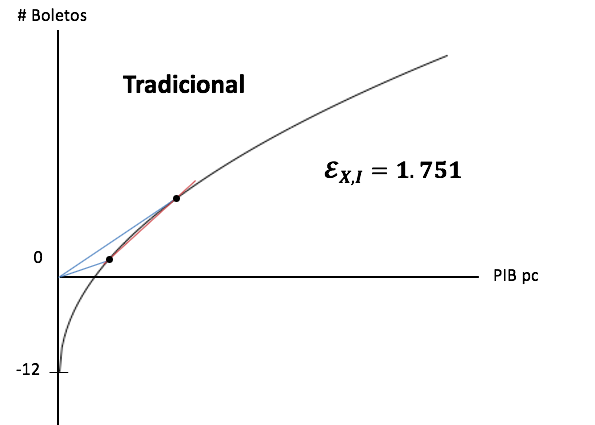
\includegraphics[width=.45\linewidth]{Imagenes/trad.png}
\end{subfigure}
\end{figure}

\newpage

Por otro lado, el coeficiente $\beta_2$ nos dice si la función es cóncava o convexa. Como se mencionó anteriormente, un individuo que es averso al riesgo tiene preferencias cóncavas ($U^{\prime \prime} < 0$). Para todos los sorteos el coeficiente $\beta_2$ es negativo pero muy cercano a cero, lo cual nos dice que los individuos son aversos al riesgo aunque la relación es casi lineal, consistente con el hecho que los bienes son superiores al ingreso. Además, al aumentar el ingreso la curva de utilidad se aplana lo cual implica que la curva es cóncava. Lo anterior nos vuelve a confirmar que los individuos que participan en estas loterías son aversos al riesgo. \\

\begin{figure}[H]
    \centering
    \caption{Relación \beta_2}
    \label{fig:my_label}
    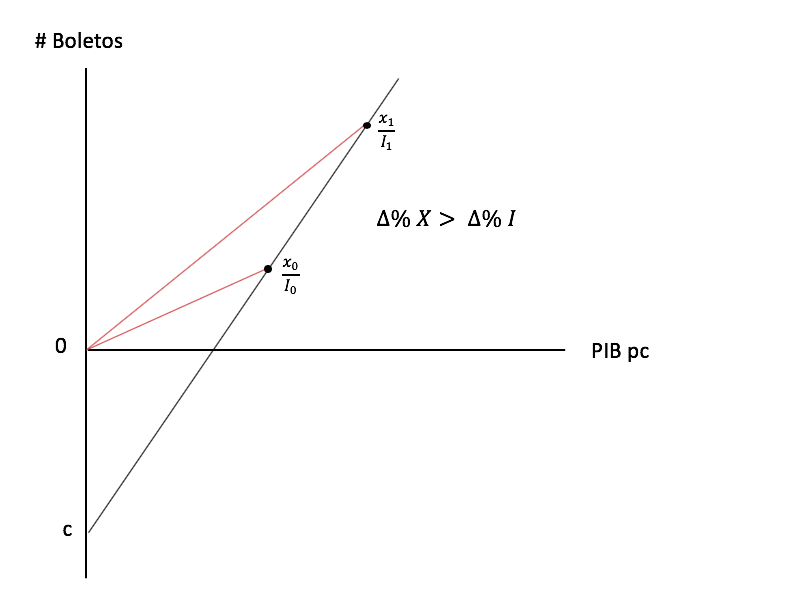
\includegraphics[width=.85\linewidth]{Imagenes/sorteo_gen2.png}
\end{figure} \\

\newpage

%Checar si esto lo puedo poner en otra parte


Se obtuvo información\footnote{Información publicada el 22 de abril de 2020 en la platorma EIKON} sobre las estimaciones del PIB para 2020 de 35 diferentes instituciones, dichas instituciones publican la variación anual que tendrá el PIB para finales del 2020. De las diferentes publicaciones un punto importante a mencionar es que ninguna institución (de las enlistadas) prevee algún crecimiento del PIB para 2020, todas las estimaciones son negativas con un promedio de -5.3 \%, una mínima de -8.0 \% por parte de \textit{Bank of America} y una máxima de -2.0 \% por parte de \textit{Julius Baer}. \\

Usamos esta información para tomarla como el $\Delta \% PIB$ y con el cálculo previo de la elasticidad ingreso para cada sorteo se calculó el $\Delta \%  \: cantidad \: de \: boletos$, que estimamos será la disminución para 2020 en la venta de boletos del Sorteo Tec. \\

%Arreglar el tamaño de la tabla 
\begin{table}[H]
\caption{Resumen $\Delta \%$ número de boletos}
\label{tab:my-resDx}
\begin{tabular}{l|l|llll}
           & $\Delta$ \% PIB   & AventuraT & Mi Sueño & Educativo & Tradicional \\ \hline
Media      & -5.3 & -8.25     & -9.92    & -9.23     & -9.37       \\
Min (BofA) & -8.0 & -12.34    & -14.83   & -13.81    & -14.01      \\
Max (JB)   & -2.0 & -3.08     & -3.71    & -3.45     & -3.50       \\ \hline
\end{tabular}
\end{table}

Observamos que, en promedio, la disminución de venta de boletos del Sorteo Tec estará entre 8\% y 9\%. El sorteo Mi Sueño es donde se podría observar una mayor disminución en el porcentaje de ventas bajo el supuesto de \textit{Bank of America}. Bajo el supuesto de \textit{Julius Baer} de nuevo el sorteo Mi Sueño es el que se vería más afectado. A continuación, presentamos los resultados bajo los escenarios previstos para las 35 instituciones.

\begin{table}[H]
\centering
\caption{Resultados para diferentes escenarios}
\label{}
\scalebox{0.7}{
\begin{tabular}{l|l|llll}
                                 & \multicolumn{1}{c|}{$\Delta$ \% PIB} & \multicolumn{4}{c}{\textit{\textbf{$\Delta$ \% cantidad boletos}}}                                                                                       \\ \hline
\multicolumn{1}{c|}{Institución} & \multicolumn{1}{c|}{2020}   & \multicolumn{1}{c}{AventuraT} & \multicolumn{1}{c}{Mi Sueño} & \multicolumn{1}{c}{Educativo} & \multicolumn{1}{c}{Tradicional} \\ \hline
ABN AMRO                         & -6                          & -9.3                          & -11.1                        & -10.4                         & -10.5                           \\
Actinver                         & -6.2                        & -9.6                          & -11.5                        & -10.7                         & -10.9                           \\
Banco Base                       & -8                          & -12.3                         & -14.8                        & -13.8                         & -14.0                           \\
Banorte                          & -7.8                        & -12.0                         & -14.5                        & -13.5                         & -13.7                           \\
Barclays                         & -5                          & -7.7                          & -9.3                         & -8.6                          & -8.8                            \\
BayernLB                         & -2.5                        & -3.9                          & -4.6                         & -4.3                          & -4.4                            \\
BofAML                           & -8                          & -12.3                         & -14.8                        & -13.8                         & -14.0                           \\
BBVA                           & -7                          & -10.8                         & -13.0                        & -12.1                         & -12.3                           \\
CaixaBank                        & -5                          & -7.7                          & -9.3                         & -8.6                          & -8.8                            \\
Capital Econ                     & -6                          & -9.3                          & -11.1                        & -10.4                         & -10.5                           \\
Citigroup                        & -5.1                        & -7.9                          & -9.5                         & -8.8                          & -8.9                            \\
Continuum Econ                   & -5.5                        & -8.5                          & -10.2                        & -9.5                          & -9.6                            \\
Credit Suisse                    & -4                          & -6.2                          & -7.4                         & -6.9                          & -7.0                            \\
DZ Bank                          & -6.5                        & -10.0                          & -12.1                        & -11.2                         & -11.4                           \\
Fitch Rating                     & -4                          & -6.2                          & -7.4                         & -6.9                          & -7.0                            \\
Goldman Sachs                    & -4.3                        & -6.6                          & -8.0                         & -7.4                          & -7.5                            \\
ING Fin Mkts                     & -3.8                        & -5.9                          & -7.0                         & -6.6                          & -6.7                            \\
Invex                            & -6                          & -9.3                          & -11.1                        & -10.4                         & -10.5                           \\
JP Morgan                        & -7.5                        & -11.6                         & -13.9                        & -12.9                         & -13.1                           \\
Julius Baer                      & -2                          & -3.1                          & -3.7                         & -3.5                          & -3.5                            \\
Moodys Investors Service         & -3.7                        & -5.7                          & -6.9                         & -6.4                          & -6.5                            \\
Morgan Stanley                   & -7.2                        & -11.1                         & -13.3                        & -12.4                         & -12.6                           \\
NORD/LB                          & -4.5                        & -6.9                          & -8.3                         & -7.8                          & -7.9                            \\
Natixis                          & -4                          & -6.2                          & -7.4                         & -6.9                          & -7.0                            \\
Nomura                           & -3.5                        & -5.4                          & -6.5                         & -6.0                          & -6.1                            \\
Pantheon                         & -5                          & -7.7                          & -9.3                         & -8.6                          & -8.8                            \\
Rabobank                         & -6.8                        & -10.5                         & -12.6                        & -11.7                         & -11.9                           \\
S\&P                             & -6.7                        & -10.3                         & -12.4                        & -11.6                         & -11.7                           \\
Scotiabank                       & -5.8                        & -8.9                          & -10.8                        & -10.0                         & -10.2                           \\
Signum Research                  & -6.8                        & -10.5                         & -12.6                        & -11.7                         & -11.9                           \\
Societe Generale                 & -3.2                        & -4.9                          & -5.9                         & -5.5                          & -5.6                            \\
Standard Chartered               & -2.9                        & -4.5                          & -5.4                         & -5.0                          & -5.1                            \\
UBS                              & -7.6                        & -11.7                         & -14.1                        & -13.1                         & -13.3                           \\
Ve Por Mas                       & -4.2                        & -6.5                          & -7.8                         & -7.2                          & -7.4                            \\
Wells Fargo                      & -5.1                        & -7.9                          & -9.5                         & -8.8                          & -8.9                            \\ \hline
\end{tabular}
}
\end{table}

\newpage

Con los resultados obtenidos, es importante aclarar diferentes puntos. Las predicciones de la caida de boletos vendidos sólo responde a la caída en el PIB. Esto es el efecto ingreso, pues la elasticidad es precisamente lo que mide \textit{ceteris paribus}. A esta caída se le deben de sumar otros efectos, tales como la menor promoción que habrá de los boletos debido al "quédate en casa"; es muy probable que mucha gente pierda su fuente ingreso; las visitas a la Casa Tec generan muchas ventas, debido a la pandemia el inmueble está cerrado y así las ventas no se generan y por último, no hay gente en el campus. Otro aspecto a considerar es el problema que se genera en la distribución de los boletos y la recolección de pagos y talones de los clientes que aun prefieren el boleto físico al digital. Todos estos factores deben de ser tomados en cuenta para entender la dimensión de la disminución en la venta de boletos. 

\chapter*{Conclusiones}
\addcontentsline{toc}{chapter}{Conclusiones}

% Las conclusiones tampoco cuentan como capítulo

\noindent Desde el primer estudio formal de la aversión al riesgo con Bernoulli en el análisis de las apuestas con la paradoja de San Petersburgo en el siglo XVII, un gran número de estudios se han desarrollado con el paso de los años. Esto con la finalidad de entender el proceso de decisión al que se enfrentan los individuos en la toma de decisiones y el por qué varía tanto entre estos. \\

Se analizaron cuatro diferentes loterías del Sorteo Tec, cada uno con diferentes premios, números de boletos vendidos, precios y por ende diferentes probabilidades de ganar algún premio. A pesar de lo anterior, los resultados obtenidos para los cuatro sorteos fueron muy similares. \\

Para esta tesis, se utilizaron modelos econométricos para la estimación de la elasticidad ingreso y la obtención de la concavidad o convexidad de la función de utilidad. Se realizó un estudio de análisis de sensibilidad de la demanda de boletos de estos diferentes sorteos. Se buscó la relación existente con el ingreso de los individuos para así determinar qué tipo de bienes son. \\

Para los cuatro sorteos que se estudiaron, se obtuvo que son bienes \textbf{superiores al ingreso} ($\varepsilon_{X,I} > 1$). Este resultado es uno de los más importantes pues, al comparar frente a los diversos resultados en la literatura relacionada a la estimación de la elasticidad ingreso de boletos de lotería, la mayoría arrojan que son bienes normales al ingreso ($0 < \varepsilon_{X,I} < 1$). De esta forma, al ser los boletos de los cuatro sorteos bienes superiores al ingreso, el efecto que resulta de un cambio en el ingreso a la cantidad demandada de estos bienes es mayor. \\

En adición a lo anterior, los resultados revelaron que la función de utilidad que representa a los jugadores de estas loterías es cóncava, esto es $U^{\prime \prime} < 0$, aunque esta relación no es tan fuerte debido a que el coeficiente que nos indica esta relación es muy cercana a cero para los cuatro sorteos. De esta manera, podemos concluir que los individuos que participn en estas loterías son \textbf{aversos al riesgo}. Lo que se pierde por comprar el boleto es poco en relación al ingreso inicial con el que cuentan los individuos. Esto implica que los individuos no requieren de una alta probabilidad de ganar un premio para decidir comprar un boleto. Es importante mencionar que el valor esperado de las cuatro loterías es menor al precio de entrada que se paga por particapar en estas apuestas. \\ 

Para los organizadores del Sorteo Tec estos son resultados un tanto ambiguos pues dependerá de la situación en que se encuentre el ingreso de los consumidores. Bajo nuestra hipótesis, en situaciones de crisis económica como la que se está viviendo al momento de escribir esta tesis (recesión, coronavirus, incertidumbre jurídica por parte del Ejecutivo, etc.) la disminución en la venta de boletos no va a ser lineal sino cada vez será mayor. \\

El escenario macroeconómico para el 2020 no figura bien. La economía mexicana ha venido a la baja desde 2019, esto se debe a diferentes factores tanto internos como externos. A lo largo del año diferentes instituciones han publicado sus estimaciones del PIB para 2020, la tendencia a lo largo del año hasta abril del 2020 ha sido recortar estas estimaciones. Bajo los escenarios presentados por estas diferentes instituciones hasta abril, se observa que el impacto en la disminución en el número de boletos vendidos será de una magnitud considerable. Las predicciones muestran disminuciones desde un -3\% hasta un -14\% \\

Con los resultados obtenidos, nuestra hipótesis se sustenta de forma tal que, ante situaciones de crisis económica, el número de boletos vendidos por el Sorteo Tec será menor. El impacto será mayor que la caida en el PIB y esta relación no será lineal. \\

%FALTA ESCRIBIR MAS



Sería interesante para futuras investigaciones realizar un estudio que tome en consideración micro-datos de los participantes de esta lotería para poder tener una mayor descripción de los participantes y ver cómo es la asignación de recursos en cada sector de la población tomando en cuenta variables geográficas, demográficas, ingreso y niveles de educación.




%----------------------------------------------------------------------------------------
%	APÉNDICES
%----------------------------------------------------------------------------------------

\begin{appendix}

\chapter{Validación modelos econométricos}

Se presentan a continuación las validaciones de los modelos econométricos que se ajustaron. Es todos los casos el análisis de residuales fue satisfactorio y no hubo que transformar las variables para corregir algún problema. Para la gráfica de residuales vs ajustados no se observa alguna tendencia y los puntos se ven aleatorios, por este motivo no vemos la existencia de problemas de heterocedasticidad. Además, los residuales siguen una distribución normal por como se ve el QQ-Plot. Por otro lado, en ningún modelo se encontró problemas con datos influyentes o atípicos. 

\newpage

\begin{figure}[H]
\centering
\label{fig:Validacion}
\begin{subfigure}
  \centering
  \caption{Validación modelo AventuraT}
  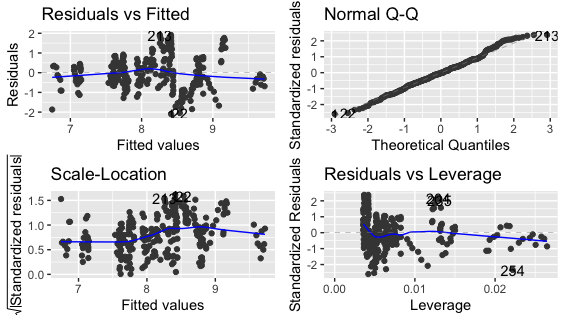
\includegraphics[width=.85\linewidth]{Imagenes/log_avent.png}
\end{subfigure}%
\begin{subfigure}
  \centering
  \caption{Validación modelo Educativo}
  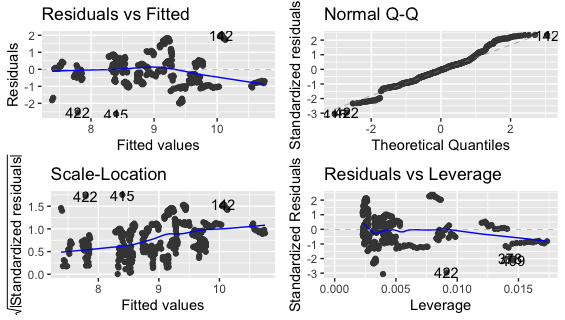
\includegraphics[width=.85\linewidth]{Imagenes/log_educ.png}
\end{subfigure}
\end{figure}

\begin{figure}[H]
\centering
\label{fig:Validacion2}
\begin{subfigure}
  \centering
  \caption{Validación modelo Mi Sueño}
  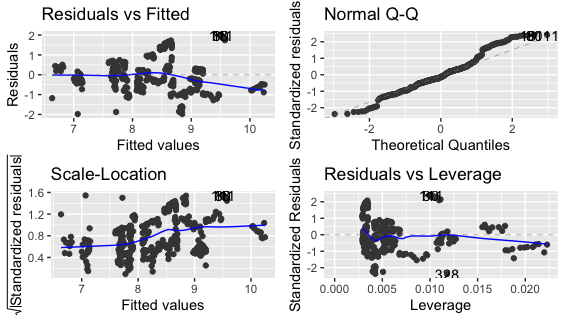
\includegraphics[width=.85\linewidth]{Imagenes/log_suen.png}
\end{subfigure}%
\begin{subfigure}
  \centering
  \caption{Validación modelo Tradicional}
  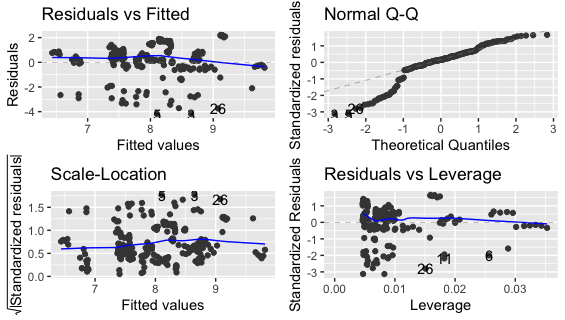
\includegraphics[width=.85\linewidth]{Imagenes/log_trad.png}
\end{subfigure}
\end{figure}

\noindent 

\chapter{Validación modelo (3.2)}

Se presenta a continuación la validación del modelo (3.2) que se aplicó a los 3 sorteos. Se observa que para todos los sorteos el modelo ajustado cumple con los supuestos de una regresión lineal múltiple. En las gráficas \textbf{\textit{Residuals vs Fitted}} no se observa alguna tendencia y los puntos se ven aleatorios, de esta forma no observamos la existencia de problemas de heterocedasticidad. En las gráficas \textbf{\textit{Normal Q-Q}} observamos que los cuantiles de los residuales están alineados con los cuantiles teóricos de una distribución normal. Por otro lado, en ningún modelo se encontraron datos influyentes o atípicos.

\begin{figure}[H]
\centering
\label{fig:Validacion_mod2}
\begin{subfigure}
  \centering
  \caption{Validación modelo (3.2) AventuraT}
  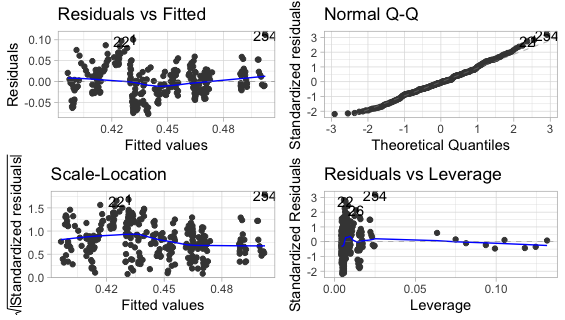
\includegraphics[width=.85\linewidth]{Imagenes/cuadritco_aven.png}
\end{subfigure}%
\begin{subfigure}
  \centering
  \caption{Validación modelo (3.2) Educativo}
  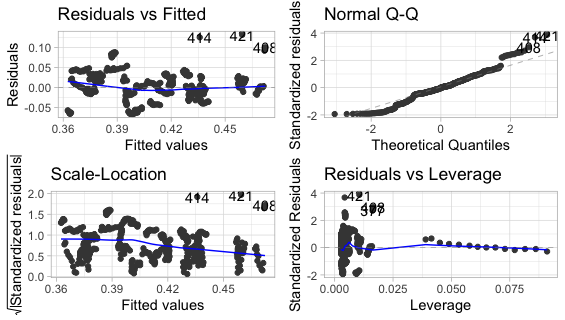
\includegraphics[width=.85\linewidth]{Imagenes/cuadratico_educ.png}
\end{subfigure}
\end{figure}

\begin{figure}[H]
\centering
\label{fig:Validacion_modelo2}
\begin{subfigure}
  \centering
  \caption{Validación modelo (3.2) Mi Sueño}
  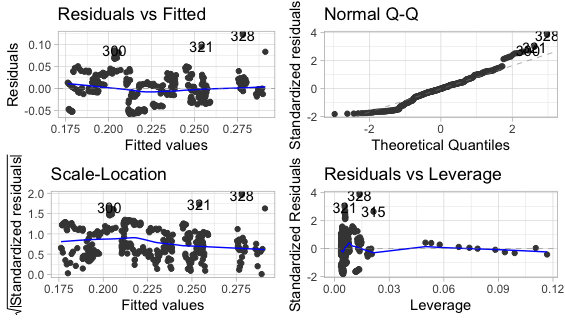
\includegraphics[width=.85\linewidth]{Imagenes/cuadratico_suen.png}
\end{subfigure}%
\end{figure}

De igual forma, se aplicó la prueba Jarque-Bera para probar la normalidad en los residuales. Se obtivieron los siguientes resultados:

%------Tabla

\begin{table}[H]
\centering
\begin{tabular}{@{}lrrlr@{}}
\toprule
\multicolumn{5}{c}{Jarque-Bera Test}                                                                \\ \midrule
\multicolumn{1}{c}{Sorteo} & \multicolumn{1}{c}{} & \multicolumn{1}{c}{Estadístico JB} &  & p-value \\ \midrule
AventuraT                  &                      & 0.35167                            &  & 0.821  \\
Educativo                  &                      & 2.2201                             &  & 0.2685   \\
Mi Sueño                   &                      & 3.4852                             &  & 0.1315   \\ \bottomrule
\end{tabular}
\end{table}

%---------

De esta forma, observamos que los modelos son válidos y justifican estadísticamente la utilización de los coeficientes estimados por el modelo (3.2) utilizados en esta tesis.

\end{appendix}

%----------------------------------------------------------------------------------------
%	BIBLIOGRAFÍA
%----------------------------------------------------------------------------------------


\chapter*{Referencias}
\addcontentsline{toc}{chapter}{Referencias}

% Macro. Esto es muy importante, no lo borren

\makeatletter
\renewenvironment{thebibliography}[1]
     {\@mkboth{\MakeUppercase\refname}{\MakeUppercase\refname}%
      \list{}%
           {\setlength{\labelwidth}{0pt}%
            \setlength{\labelsep}{0pt}%
            \setlength{\leftmargin}{\parindent}%
            \setlength{\itemindent}{-\parindent}%
            \@openbib@code
            \usecounter{enumiv}}%
      \sloppy
      \clubpenalty4000
      \@clubpenalty \clubpenalty
      \widowpenalty4000%
      \sfcode`\.\@m}
     {\def\@noitemerr
       {\@latex@warning{Empty `thebibliography' environment}}%
      \endlist}
\makeatother

\begin{thebibliography}{111}

% Lista

% La manera recomendada para citar papers o libros en el formato de Chicago esta en el siguiente vínculo: https://www.chicagomanualofstyle.org/tools_citationguide/citation-guide-2.html

% Es importante poner el apellido del autor seguido del año de publicación, una coma y las páginas consultadas en el texto antes de puntuar y entre paréntesis para las citas en el cuerpo de la tesis

% Ejemplo:

% Las \textit{causas próximas} del crecimiento son conocidas: tecnología, capital humano y físico. La pregunta es ¿por qué unos países sí tienen estas causas próximas y otros no? La respuesta son las \textit{causas fundamentales:} suerte, geografía, cultura e instituciones (Acemoglu 2009, 110).

%AAAAA

\bibitem{Bernoulli} Bernoulli, D. (1954). \textit{Exposition of a New Theory on the Measurement of Risk}. Econometrica, 22(1), 23–36.

\bibitem{salRisk} Bordalo, P., Gennaioli, N., \& Shleifer, A. (2010). \textit{Salience Theory of Choice Under Risk}. The Quarterly Journal of Economics, 127(3), 1243–1285.

\bibitem{housingG} Carliner, G. (1973). \textit{Income Elasticity of Housing Demand}. The Review of Economics and Statistics, 55(4), 528–532.

\bibitem{tgarret} Garrett, T. A. (2015). \textit{The (Aggregate) Demand for State Lottery Tickets: What Have We Really Learned?} Contemporary Economic Policy, 34(3), 475–482.

\bibitem{locPrice} Garrett, T. A., \& Kolesnikova, N. (2014). \textit{Local Price Variation and the Income Elasticity of Demand for Lottery Tickets}. Public Finance Review, 43(6), 717–738.

\bibitem{gujarati} Gujarati, D. N., & Porter, D. C. (2008). \textit{Basic Econometrics} (5th ed.). McGraw-Hill Education.

\bibitem{taxIn} Heavey, J. F. (1978). \textit{The Incidence of State Lottery Taxes}. Public Finance Quarterly, 6(4), 415–426.

\bibitem{masscol95} Mas-Colell, A., Whinston, M. D., \& Green, J. R. (1995). \textit{Microeconomic Theory} (1st ed.). New York, United States: Oxford University Press.

\bibitem{VonnNeu} Neumann, V. J., \& Morgenstern, O. (1953). \textit{Theory of Games and Economic Behavior} (3rd ed.). New York, United States: Princeton University Press.

\bibitem{nich10} Nicholson, W., \& Snyder, C. (2007). \textit{Microeconomic Theory: Basic Principles and Extensions}. Ohio, United States: Cengage Learning.

\bibitem{oDon} O’Donoghue, T., \& Somerville, J. (2018). \textit{Modeling Risk Aversion in Economics}. Journal of Economic Perspectives, 32(2), 91–114.

\bibitem{OsterE} Oster, E. (2004). \textit{Are All Lotteries Regressive? Evidence from the Powerball}. National Tax Journal, 57(2), 179–187.

\bibitem{lotSpain} Pérez, L., \& Humphreys, B. R. (2011). \textit{The Income Elasticity of Lottery: New Evidence from Micro Data}. Public Finance Review, 39(4), 551–570. 

\bibitem{pratt} Pratt, J. W. (1964). \textit{Risk Aversion in the Small and in the Large}. Econometrica, 32(1/2), 122–136. 

\bibitem{sppiro} Spiro, M. H. (1974). \textit{On the Tax Incidence of the Pennsylvania Lottery}. National Tax Journal, 27(1), 57–61. 









%BBBBB

%CCCCC

%DDDDD

%EEEEE

%FFFFF

%GGGGG

%HHHHH

%IIIII

%JJJJJ

%KKKKK

%LLLLL

%MMMMM

%NNNNN

%OOOOO

%PPPPP

%QQQQQ

%RRRRR

%SSSSS

%TTTTT

%UUUUU

%VVVVV

%WWWWW

%XXXXX

%YYYYY

%ZZZZZ

\end{thebibliography}

\newpage
\thispagestyle{empty}
\begin{table}[p]
\centering
\small
\label{ed}
\begin{tabular}{c}
\textit{Risk is a matter of knowledge,}\\ \textit{not perception.}\\
escrito por Luis Irán Vázquez López,\\ se terminó de imprimir en mes de año\\ en los talleres de Tesis Matozo.\\ Campeche 156, colonia Roma,\\ Ciudad de México.
\end{tabular}
\end{table}

% Si lo prefieren, avisen a su taller que esta página ya la incluyeron ustedes para que no les impriman las que ellos usan. Lo recomiendo ampliamente

%%%%%%%%%%%%%%%%%%%%%%%%%%%%%%%%%%%%%%%%%%%%%%%%%%%%%%%%%%%%%%%%%%%%%%%%%%%%%%%%%%%%%%%

\end{document}